% LaTeX source for ``Complexity and Computation''
% Copyright (c)  2011  Allen B. Downey.

% Permission is granted to copy, distribute, transmit and adapt
% this work under a Creative Commons 
% Attribution-NonCommercial-ShareAlike 3.0 Unported License:
% http://creativecommons.org/licenses/by-nc-sa/3.0/

% If you are interested in distributing a commercial version of this
% work, please contact Allen B. Downey.

% The LaTeX source for this book is available from
% http://greenteapress.com/complexity
% http://code.google.com/p/complexity

% This book was typeset using LaTeX .  The illustrations were
% drawn in xfig.  All of these are free, open-source programs.

%%----------------------------------------------------------------

% How to compile this document:
% If your environment provides latex, makeindex, and dvips,
% the following commands should produce a Postscript version
% of the book.

%        latex book
%        makeindex book
%        latex book
%        dvips -o book.ps book

% You will also need the following (fairly standard) latex
% packages: url, epsfig, makeidx, fancyhdr

% This distribution also includes a Makefile that should
% compile both the Postscript and PDF versions of the book.

%%-----------------------------------------------------------------

\documentclass[10pt]{book}
\usepackage[width=5.5in,height=8.0in,
  hmarginratio=3:2,vmarginratio=1:1]{geometry}

\usepackage{url}
\usepackage{fancyhdr}
\usepackage{graphicx}
\usepackage{amsmath, amsthm, amssymb}
\usepackage{exercise}
\usepackage{makeidx}
\usepackage{setspace}
\usepackage{hevea}
\usepackage{upquote}

\newcommand{\thetitle}{Complexity and Computation}
\newcommand{\theversion}{0.9.1}

\makeindex

\begin{document}

\frontmatter

% LATEXONLY

\input{latexonly}

\newtheorem{ex}{Exercise}[chapter]

\begin{latexonly}

\renewcommand{\blankpage}{\thispagestyle{empty} \quad \newpage}

%\blankpage
%\blankpage

% TITLE PAGES FOR LATEX VERSION

%-half title--------------------------------------------------
\thispagestyle{empty}

\begin{flushright}
\vspace*{2.0in}

\begin{spacing}{3}
{\huge \thetitle}
\end{spacing}

\vspace{0.25in}

Version \theversion

\vfill

\end{flushright}

%--verso------------------------------------------------------

\blankpage
\blankpage
%\clearemptydoublepage
%\pagebreak
%\thispagestyle{empty}
%\vspace*{6in}

%--title page--------------------------------------------------
\pagebreak
\thispagestyle{empty}

\begin{flushright}
\vspace*{2.0in}

\begin{spacing}{3}
{\huge \thetitle}
\end{spacing}

\vspace{0.25in}

Version \theversion

\vspace{1in}


{\Large
Allen Downey\\
}


\vspace{0.5in}

{\Large Green Tea Press}

{\small Needham, Massachusetts}

%\includegraphics[width=1in]{figs/logo1.eps}
\vfill

\end{flushright}


%--copyright--------------------------------------------------
\pagebreak
\thispagestyle{empty}

{\small
Copyright \copyright ~2011 Allen Downey.


Printing history:

\begin{description}

\item[Fall 2008:] First edition.

\item[Fall 2011:] Second edition.

\end{description}

\vspace{0.2in}

\begin{flushleft}
Green Tea Press       \\
9 Washburn Ave \\
Needham MA 02492
\end{flushleft}

Permission is granted to copy, distribute, transmit and adapt
this work under a Creative Commons 
Attribution-NonCommercial-ShareAlike 3.0 Unported License:
\url{http://creativecommons.org/licenses/by-nc-sa/3.0/}.

If you are interested in distributing a commercial version of this
work, please contact Allen B. Downey.

The original form of this book is \LaTeX\ source code.  Compiling this
\LaTeX\ source has the effect of generating a device-independent
representation of the book, which can be converted to other formats
and printed.

The \LaTeX\ source for this book is available from

\begin{verbatim}
      http://greenteapress.com/complexity
      http://code.google.com/p/complexity
\end{verbatim}

This book was typeset using \LaTeX .  The illustrations were
drawn in xfig.

\vspace{0.2in}

} % end small

\end{latexonly}


% HTMLONLY

\begin{htmlonly}

% TITLE PAGE FOR HTML VERSION

{\Large \thetitle}

{\large Allen B. Downey}

Version \theversion

\setcounter{chapter}{-1}

\end{htmlonly}

\chapter{Preface}

This book is about data structures and algorithms, intermediate
programming in Python, computational modeling and
the philosophy of science:

\begin{description}

\item[Data structures and algorithms:] A data structure is a
  collection of data elements organized in a way that supports
  particular operations.  For example, a Python dictionary organizes
  key-value pairs in a way that provides fast mapping from keys to
  values, but mapping from values to keys is slower.

An algorithm is a mechanical process for performing a computation.
Designing efficient programs often involves the co-evolution of data
structures and the algorithms that use them.  For example, in the
first few chapters I will present graphs, data structures that
implement graphs, and graph algorithms based on those data structures.

\item[Python programming:] This book picks up where {\em Think Python}
  leaves off.  I assume that you have read that book or have
  equivalent knowledge of Python.  I try to emphasize fundmental ideas
  that apply to programming in many languages, but along the way you
  will learn some useful features that are specific to Python.

\item[Computational modeling:] A model of a system is a simplified
  description of a system used for simulation or analysis.
  Computational models are designed to take advantage of cheap, fast
  computation.

\item[Philosophy of science:] The models and results in this book
  raise questions relevant to the philosophy of science,
  including the nature of scientific laws, theory choice, realism and
  instrumentalism, holism and reductionism, and epistemology.

\end{description}

There are two kinds of computational models:

\begin{description}

\item[Continuous:] Many computational models compute approximate
  solutions to equations that are continuous in space and time.  For
  example, to compute the trajectory of a planet, you could describe
  planetary motion using differential equations and then compute the
  position of the planet at discrete points in time.

The fields of numerical methods and scientific computing
tend to focus on these kinds of models.

\item[Discrete:] Discrete models include graphs, cellular automata,
  and agent-based models.  They are often characterized by structure,
  rules and transitions rather than by equations.  They tend to be
  more abstract than continuous models; in some cases there is no
  direct correspondence between the model and a physical system.

\end{description}

Complexity science is an interdiscipinary field---at the intersection
of mathematics, computer science and natural science---that focuses on
discrete models of physical systems.

And that's what this book is about.


Allen B. Downey \\
Needham MA\\

Allen Downey is a Professor of Computer Science at 
the Franklin W. Olin College of Engineering.




\section*{Contributor List}

\index{contributors}

If you have a suggestion or correction, please send email to 
{\tt downey@greenteapress.com}.  If I make a change based on your
feedback, I will add you to the contributor list
(unless you ask to be omitted).

If you include at least part of the sentence the
error appears in, that makes it easy for me to search.  Page and
section numbers are fine, too, but not quite as easy to work with.
Thanks!

\small

\begin{itemize}

\item Richard Hollands pointed out several typos.

\item John Harley, Jeff Stanton, Colden Rouleau and
Keerthik Omanakuttan are Computational Modeling students who
pointed out typos.

\item Muhammad Najmi bin Ahmad Zabidi caught some typos.


% ENDCONTRIB

\end{itemize}

\normalsize

\clearemptydoublepage

% TABLE OF CONTENTS
\begin{latexonly}

\tableofcontents

\clearemptydoublepage

\end{latexonly}

% START THE BOOK
\mainmatter


\chapter{Graphs}

\section{What's a graph?}

To most people a graph is a visual representation of a data set, like
a bar chart or an EKG.  That's not what this chapter is about.

In this chapter, a {\bf graph} is an abstraction used to
model a system that contains discrete, interconnected elements.  The
elements are represented by {\bf nodes} (also called {\bf vertices})
and the interconnections are represented by {\bf edges}.

For example, you could represent a road map with one node for each
city and one edge for each road between cities.  Or you could
represent a social network using one node for each person, with an
edge between two people if they are ``friends'' and no edge otherwise.

In some graphs, edges have different lengths (sometimes
called ``weights'' or ``costs'').  For example, in a road map, the
length of an edge might represent the distance between
two cities, or the travel time, or bus fare.
In a social network there might be different kinds of
edges to represent different kinds of relationships: friends,
business associates, etc.

Edges may be {\bf undirected}, if they representation a relationship
that is symmetric, or {\bf directed}.  In a social network,
friendship is usually symmetric: if $A$ is friends with $B$ then
$B$ is friends with $A$.  So you would probably represent friendship
with an undirected edge.  In a road map, you would probably represent
a one-way street with a directed edge.

Graphs have interesting mathematical properties, and
there is a branch of mathematics called {\bf graph theory}
that studies them.

Graphs are also useful, because there are many real world
problems that can be solved using {\bf graph algorithms}.
For example, Dijkstra's shortest path algorithm is an efficient
way to find the shortest path from a node to all
other nodes in a graph.  A {\bf path} is a sequence of nodes
with an edge between each consecutive pair.

Sometimes the connection between a real world problem and
a graph algorithm is obvious.  In the road map example, it is
not hard to imagine using a shortest path algorithm to find
the route between two cities that minimizes distance (or time,
or cost).

In other cases it takes more effort to represent a problem in a form
that can be solved with a graph algorithm, and then interpret the
solution.

For example, a complex system of radioactive decay
can be represented by a
graph with one node for each nuclide (type of atom) and an edge
between two nuclides if one can decay into the other.  A path in this
graph represents a decay chain.
See \url{wikipedia.org/wiki/Radioactive_decay}.

The rate of decay between two nuclides is characterized by a decay
constant, $\lambda$, measured in becquerels (Bq) or decay events per
second.  You might be more familiar with half-life, $t_{1/2}$, which
is the expected time until half of a sample decays.  You can convert
from one characterization to the other using the relation $t_{1/2} =
\ln 2 / \lambda$.

In our best current model of physics, nuclear decay is a fundamentally
random process, so it is impossible to predict when an atom will
decay.  However, given $\lambda$, the probability that an atom will
decay during a short time interval $dt$ is $\lambda dt$.

In a graph with multiple decay chains, the probability of a
given path is the product of the probabilities of each decay
process in the path.

Now suppose you want to find the decay chain with the highest
probability.  You could do it by assigning each edge a ``length'' of
$-\log \lambda$ and using a shortest path algorithm.  Why?  Because the
shortest path algorithm adds up the lengths of the edges, and adding
up log-probabilities is the same as multiplying probabilities.  Also,
because the logarithms are negated, the smallest sum corresponds to
the largest probability.  So the shortest path corresponds to the most
likely decay chain.

This is an example of a common and useful process in applying
graph algorithms:

\begin{description}

\item[Reduce] a real-world problem to an instance of a graph
problem.
 
\item[Apply] a graph algorithm to compute the result efficiently.

\item[Interpret] the result of the computation in terms of a
solution to the original problem.

\end{description}

We will see other examples of this process soon.

\begin{ex}

Read the Wikipedia page about graphs at
\url{http://en.wikipedia.org/wiki/Graph_(mathematics)}
and answer the following questions:

\begin{enumerate}

\item What is a simple graph?  In the rest of this section,
we will be assuming that all graphs are simple graphs.  This
is a common assumption for many graph algorithms---so
common it is often unstated.

\item What is a regular graph?  What is a complete graph?  Prove
that a complete graph is regular.

\item What is a path?  What is a cycle?

\item What is a forest?  What is a tree?  Note: a graph
is {\bf connected} if there is a path from every node to
every other node.

\end{enumerate}

\end{ex}



\section{Representing graphs}

Graphs are usually drawn with squares or circles for nodes and lines
for edges.  In the example below, the graph on the left represents
a social network with three people.

%A set of nodes like this,
%where each node is connected to all of the others, is called
%a {\bf clique} (pronounced ``cleek'').

\beforefig
\centerline{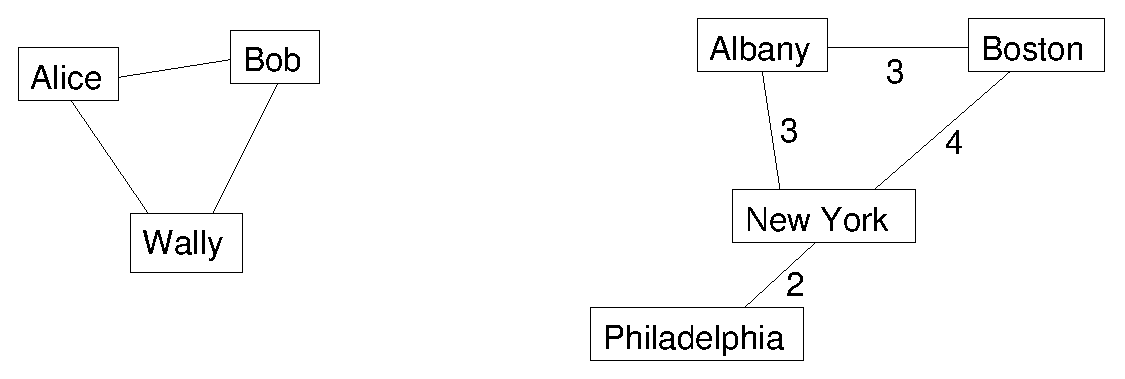
\includegraphics[width=5.5in]{figs/graph_examples.eps}}
\afterfig

In the graph on the right, the weights of the edges are the
approximate travel times, in hours, between cities in the northeast
United States.  In this case the placement of the nodes corresponds
roughly to the geography of the cities, but in general the layout
of a graph is arbitrary.

To implement graph algorithms, you have to figure
out how to represent a graph in the form of a data structure.
But to choose the best data structure, you have to know which
operations the graph should support.

To get out of this chicken-and-egg problem, I am going to present
a data structure that is a good choice for many graph algorithms.
Later we will come back and evaluate its pros and cons.

Here is an implementation of a graph as a dictionary of dictionaries:

\begin{verbatim}
class Graph(dict):
    def __init__(self, vs=[], es=[]):
        """create a new graph.  (vs) is a list of vertices;
        (es) is a list of edges."""
        for v in vs:
            self.add_vertex(v)
            
        for e in es:
            self.add_edge(e)

    def add_vertex(self, v):
        """add (v) to the graph"""
        self[v] = {}

    def add_edge(self, e):
        """add (e) to the graph by adding an entry in both directions.

        If there is already an edge connecting these Vertices, the
        new edge replaces it.
        """
        v, w = e
        self[v][w] = e
        self[w][v] = e
\end{verbatim}

The first line declares that {\tt Graph} inherits from the built-in
type {\tt dict}, so a Graph object has all the methods and operators
of a dictionary.

More specifically, a Graph is a dictionary that maps from
a Vertex $v$ to an inner dictionary that maps from a Vertex $w$
to an Edge that connects $v$ and $w$.  So if {\tt g} is a graph,
{\tt g[v][w]} maps to an Edge if there is one and raises
a {\tt KeyError} otherwise.

\verb"__init__" takes a list of vectices and a list of
edges as optional parameters.  If they are provided, it calls
\verb"add_vertex" and \verb"add_edge" to add the vertices and edges to
the graph.

Adding a vertex to a graph means making an entry for it in the
outer dictionary.  Adding an edge makes two entries, both pointing
to the same Edge.  So this implementation represents an undirected
graph.

Here is the definition for {\tt Vertex}:

\begin{verbatim}
class Vertex(object):
    def __init__(self, label=''):
        self.label = label

    def __repr__(self):
        return 'Vertex(%s)' % repr(self.label)

    __str__ = __repr__
\end{verbatim}

A Vertex is just an object that has a label attribute.  We can
add attributes later, as needed.

\verb"__repr__" is a special function that returns a string
representation of an object.  It is similar to \verb"__str__" except
that the return value from \verb"__str__" is intended to be readable
for people, and the return value from \verb"__repr__" is supposed to
be a legal Python expression.

The built-in function {\tt str} invokes \verb"__str__" on
an object; similarly the built-in function {\tt repr} invokes
\verb"__repr__".

In this case \verb"Vertex.__str__" and \verb"Vertex.__repr__" refer to
the same function, so we get the same string either way.

Here is the definition for {\tt Edge}:

\begin{verbatim}
class Edge(tuple):
    def __new__(cls, *vs):
        return tuple.__new__(cls, vs)

    def __repr__(self):
        return 'Edge(%s, %s)' % (repr(self[0]), repr(self[1]))

    __str__ = __repr__
\end{verbatim}

{\tt Edge} inherits from the built-in type {\tt tuple}
and overrides the \verb"__new__" method.  When you invoke
an object constructor, Python invokes \verb"__new__" to create
the object and then \verb"__init__" to initialize the attributes.

For mutable objects it is most common to override
\verb"__init__" and use the default implementation of
\verb"__new__", but because Edges inherit from {\tt tuple}, they
are immutable, which means that you can't modify the elements
of the tuple in \verb"__init__".

By overriding \verb"__new__", we can use the {\tt *} operator to
gather the parameters and use them to initialize the elements of
the tuple.  A precondition of this method is that there should
be exactly two arguments.  A more careful implementation would
check.

Here is an example that creates two vertices and an edge:

\begin{verbatim}
    v = Vertex('v')
    w = Vertex('w')
    e = Edge(v, w)
    print e
\end{verbatim}

Inside \verb"Edge.__str__" the term {\tt self[0]} refers  
to {\tt v} and {\tt self[1]} refers to {\tt w}.  So the output
when you print {\tt e} is:

\begin{verbatim}
Edge(Vertex('v'), Vertex('w'))
\end{verbatim}

Now we can assemble the edge and vertices into a graph:

\begin{verbatim}
    g = Graph([v, w], [e])
    print g
\end{verbatim}

The output looks like this (with a little formatting):

\begin{verbatim}
{Vertex('w'): {Vertex('v'): Edge(Vertex('v'), Vertex('w'))},
 Vertex('v'): {Vertex('w'): Edge(Vertex('v'), Vertex('w'))}}
\end{verbatim}

We didn't have to write \verb"Graph.__str__"; it is inherited
from {\tt dict}.


\begin{ex}

In this exercise you write methods that will be
useful for many of the Graph algorithms that are coming up.

\begin{enumerate}

\item Download \url{thinkcomplex.com/GraphCode.py}, which
  contains the code in this chapter.  Run it as a script and make sure
  the test code in {\tt main} does what you expect.

\item Make a copy of {\tt GraphCode.py} called {\tt Graph.py}.  Add
  the following methods to {\tt Graph}, adding test code as you go.

\item Write a method named \verb"get_edge" that takes two vertices and
  returns the edge between them if it exists and {\tt None} otherwise.
  Hint: use a {\tt try} statement.

\item Write a method named \verb"remove_edge" that takes an edge and
  removes all references to it from the graph.

\item Write a method named {\tt vertices} that returns a list of the
  vertices in a graph.

\item Write a method named {\tt edges} that returns a list of edges in
  a graph.  Note that in our representation of an undirected graph
  there are two references to each edge.

\item Write a method named \verb"out_vertices" that takes a Vertex and
  returns a list of the adjacent vertices (the ones connected to the
  given node by an edge).

\item Write a method named \verb"out_edges" that takes a Vertex and
  returns a list of edges connected to the given Vertex.

\item Write a method named \verb"add_all_edges" that starts with an
  edgeless Graph and makes a complete graph by adding edges between
  all pairs of vertices.

\end{enumerate}

Test your methods by writing test code and checking the output.  Then
download \url{thinkcomplex.com/GraphWorld.py}.  GraphWorld is
a simple tool for generating visual representations of graphs.  It is
based on the World class in Swampy, so you might have to install
Swampy first: see \url{thinkpython.com/swampy}.

Read through {\tt GraphWorld.py} to get a sense of how it works.  Then
run it.  It should import your {\tt Graph.py} and then display a
complete graph with 10 vertices.

\end{ex}


\begin{ex}

Write a method named \verb"add_regular_edges" that starts with an
edgeless graph and adds edges so that every vertex has the same
degree.  The {\bf degree} of a node is the number of edges it is
connected to.

To create a regular graph with degree 2 you would do something
like this:

\begin{verbatim}
vertices = [ ... list of Vertices ... ]
g = Graph(vertices, [])
g.add_regular_edges(2)
\end{verbatim} 

It is not always possible to create a regular graph
with a given degree, so you should figure out and document the
preconditions for this method.

To test your code, you might want to create a file named
{\tt TestGraph.py} that imports {\tt Graph.py} and
{\tt GraphWorld.py}, then generates and displays the graphs
you want to test.

\end{ex}


\newcommand{\Erdos}{Erd\H{o}s}
\newcommand{\Renyi}{R\'{e}nyi}

\section{Random graphs}

A random graph is just what it sounds like: a graph with edges
generated at random.  Of course, there are many random processes that
can generate graphs, so there are many kinds of random graph.  One
interesting kind is the \Erdos-\Renyi~model, denoted $G(n,p)$, which
generates graphs with $n$ nodes, where the probability is $p$ that
there is an edge between any two nodes.  See
\url{http://en.wikipedia.org/wiki/Erdos-Renyi_model}.

\begin{ex}

Create a file named {\tt RandomGraph.py} and define a class named 
{\tt RandomGraph} that inherits from {\tt Graph} and provides a method
named \verb"add_random_edges" that takes a probability {\tt p} as a
parameter and, starting with an edgeless graph, adds edges at random
so that the probability is $p$ that there is an edge between any two
nodes.

\end{ex}


\section{Connected graphs}
\label{bfs}

A graph is {\bf connected} if there is a path from every node to every
other node.  See \url{wikipedia.org/wiki/Connectivity_(graph_theory)}.

There is a simple algorithm to check whether a graph is connected.
Start at any vertex and conduct a search
(usually a breadth-first-search or BFS), marking all the vertices you
can reach.  Then check to see whether all vertices are marked.

You can read about breadth-first-search at
\url{wikipedia.org/wiki/Breadth-first_search}.  

In general, when you process
a node, we say that you are 
{\bf visiting} it.

In a search, you visit a node
by marking it (so you can tell later that it has been visited)
then visiting any
unmarked vertices it is connected to.

In a breadth-first-search, you visit nodes in the order they are
discovered.  You can use a queue or a ``worklist'' to keep them in
order.  Here's how it works:

\begin{enumerate}

\item Start with any vertex and add it to the queue.

\item Remove a vertex from the queue and mark it.  If it is
connected to any unmarked vertices, add them to the queue.

\item If the queue is not empty, go back to Step 2.

\end{enumerate}

\begin{ex}

Write a Graph method named \verb"is_connected" that returns
{\tt True} if the Graph is connected and {\tt False} otherwise.

\end{ex}


\section{Paul \Erdos: peripatetic mathematician, speed freak}

Paul \Erdos~ was a Hungarian mathematician who spent most
of his career (from 1934 until his death in 1992) living out
of a suitcase, visiting colleagues at universities all over the
world, and authoring papers with more than 500 collaborators.

He was a notorious caffeine addict and, for the last 20 years of his
life, an enthusiastic user of amphetamines.  He attributed at least
some of his productivity to the use of these drugs; after giving them
up for a month to win a bet, he complained that the only result
was that mathematics had
been set back by a month\footnote{Much of this biography follows
\url{wikipedia.org/wiki/Paul_Erd\H{o}s}}.

In the 1960s he and Afr\'{e}d \Renyi~ wrote a series of papers 
introducing the \Erdos-\Renyi~
model of random graphs and studying their properties.

One of their most surprising results is the existence of
abrupt changes in the characteristics of random graphs as
random edges are added.  They showed that for a number of
graph properties there is a threshold value of the probability
$p$ below which the property is rare and above which is
is almost certain.  This transition is sometimes called
a ``phase change'' by analogy with physical systems that
change state at some critical value of temperature.
See \url{wikipedia.org/wiki/Phase_transition}.


\begin{ex}

One of the properties that displays this kind of transition is
connectedness.  For a given size $n$, there is a critical value,
$p^*$, such that a random graph $G(n, p)$ is unlikely to be connected
if $p < p^*$ and very likely to be connected if $p > p^*$.

Write a program that tests this result by generating random graphs for
values of $n$ and $p$ and computes the fraction of them that
are connected.

How does the abruptness of the transition depend on $n$?

You can download my solution from
\url{thinkcomplex.com/RandomGraph.py}.

\end{ex}


\section{Iterators}

If you have read the documentation of Python dictionaries,
you might have noticed the methods {\tt iterkeys}, {\tt itervalues}
and {\tt iteritems}.  These methods are similar to {\tt keys},
{\tt values} and {\tt items}, except that instead of building
a new list, they return iterators.

An {\bf iterator} is an object that provides a method named
{\tt next} that returns the next element in a sequence.  Here
is an example that creates a dictionary and uses {\tt iterkeys}
to traverse the keys.

\begin{verbatim}
>>> d = dict(a=1, b=2)
>>> iter = d.iterkeys()
>>> print iter.next()
a
>>> print iter.next()
b
>>> print iter.next()
Traceback (most recent call last):
  File "<stdin>", line 1, in <module>
StopIteration
\end{verbatim}

The first time {\tt next} is invoked, it returns the first key from
the dictionary (the order of the keys is arbitrary).  The second
time it is invoked, it returns the second element.  The third time,
and every time thereafter, it raises a {\tt StopIteration}
exception.

An iterator can be used in a {\tt for} loop; for example, the
following is a common idiom for traversing the key-value
pairs in a dictionary:

\begin{verbatim}
    for k, v in d.iteritems():
        print k, v
\end{verbatim}

In this context, {\tt iteritems} is likely to be faster than
{\tt items} because it doesn't have to build the entire list
of tuples; it reads them from the dictionary as it goes along.

But it is only safe to use the iterator methods if you do not add or
remove dictionary keys inside the loop.  Otherwise you get an
exception:

\begin{verbatim}
>>> d = dict(a=1)
>>> for k in d.iterkeys():
...     d['b'] = 2
...
RuntimeError: dictionary changed size during iteration
\end{verbatim}

Another limitation of iterators is that they do not support index
operations.

\begin{verbatim}
>>> iter = d.iterkeys()
>>> print iter[1]
TypeError: 'dictionary-keyiterator' object is unsubscriptable
\end{verbatim}

If you need indexed access, you should use {\tt keys}.
Alternatively, the Python module {\tt itertools} provides
many useful iterator functions.

A user-defined object can be used as an iterator if it
provides methods named {\tt next} and \verb"__iter__".
The following example is an iterator that always returns {\tt True}:

\begin{verbatim}
class AllTrue(object):
    def next(self):
        return True

    def __iter__(self):
        return self
\end{verbatim}

The \verb"__iter__" method for iterators returns the iterator
itself.  This protocol makes it possible to use iterators
and sequences interchangeably in many contexts.

Iterators like {\tt AllTrue} can represent an infinite sequence.
They are useful as an argument to {\tt zip}:

\begin{verbatim}
>>> print zip('abc', AllTrue())
[('a', True), ('b', True), ('c', True)]
\end{verbatim}


\section{Generators}

For many purposes the easiest way to make an iterator is to
write a {\bf generator}, which is a function that contains a
{\tt yield} statement.  {\tt yield} is similar to {\tt return},
except that the state of the running function is stored and
can be resumed.

For example, here is a generator that yields successive letters
of the alphabet:

\begin{verbatim}
def generate_letters():
    for letter in 'abc':
        yield letter
\end{verbatim}

When you call this function, the return value is an iterator:

\begin{verbatim}
>>> iter = generate_letters()
>>> print iter
<generator object at 0xb7d4ce4c>
>>> print iter.next()
a
>>> print iter.next()
b
\end{verbatim}

And you can use an iterator in a {\tt for} loop:

\begin{verbatim}
>>> for letter in generate_letters():
...     print letter
...
a
b
c
\end{verbatim}

A generator with an infinite loop returns an iterator that
never terminates.  For example, here's a generator that
cycles through the letters of the alphabet:

\begin{verbatim}
def alphabet_cycle():
    while True:
        for c in string.lowercase:
            yield c
\end{verbatim}


\begin{ex}

Write a generator that yields an infinite sequence of alpha-numeric
identifiers, starting with {\tt a1} through {\tt z1}, then {\tt a2}
through {\tt z2}, and so on.

\end{ex}


\chapter{Analysis of algorithms}

Analysis of algorithms is the branch of computer science that studies
the performance of algorithms, especially their run time and space
requirements.  See \url{wikipedia.org/wiki/Analysis_of_algorithms}.

%\url{wikipedia.org/wiki/Run-time_analysis}

The practical goal of algorithm analysis is to predict the performance
of different algorithms in order to guide design decisions.

During the 2008 United States Presidential Campaign, candidate
Barack Obama was asked to perform an impromptu analysis when
he visited Google.  Chief executive Eric Schmidt jokingly asked him
for ``the most efficient way to sort a million 32-bit integers.''
Obama had apparently been tipped off, because he quickly
replied, ``I think the bubble sort would be the wrong way to go.''
See \url{http://www.youtube.com/watch?v=k4RRi_ntQc8}.

This is true: bubble sort is conceptually simple but slow for
large datasets.  The answer Schmidt was probably looking for is
``radix sort'' (see \url{wikipedia.org/wiki/Radix_sort})\footnote{
But if you get a question like this in an interview, I think
a better answer is, ``The fastest way to sort a million integers
is to use whatever sort function is provided by the language
I'm using.  Its performance is good enough for the vast majority
of applications, but if it turned out that my application was too
slow, I would use a profiler to see where the time was being
spent.  If it looked like a faster sort algorithm would have
a significant effect on performance, then I would look
around for a good implementation of radix sort.''}.

So the goal of algorithm analysis is to make meaningful
comparisons between algorithms, but there are some problems:

\begin{itemize}

\item The relative performance of the algorithms might
depend on characteristics of the hardware, so one algorithm
might be faster on Machine A, another on Machine B.
The general solution to this problem is to specify a
{\bf machine model} and analyze the number of steps, or
operations, an algorithm requires under a given model.

\item Relative performance might depend on the details of
the dataset.  For example, some sorting
algorithms run faster if the data are already partially sorted;
other algorithms run slower in this case.
A common way to avoid this problem is to analyze the
{\bf worst case} scenario.  It is also sometimes useful to
analyze average case performance, but it is usually harder,
and sometimes it is not clear what set of cases to average over.

\item Relative performance also depends on the size of the
problem.  A sorting algorithm that is fast for small lists
might be slow for long lists.
The usual solution to this problem is to express run time
(or number of operations) as a function of problem size,
and to compare the functions {\bf asymptotically} as the problem
size increases.

\end{itemize}

The good thing about this kind of comparison that it lends
itself to simple classification of algorithms.  For example,
if I know that the run time of Algorithm A tends to be
proportional to the size of the input, $n$, and Algorithm B
tends to be proportional to $n^2$, then I
expect A to be faster than B for large values of $n$.

This kind of analysis comes with some caveats, but we'll get
to that later.


\section{Order of growth}

Suppose you have analyzed two algorithms and expressed
their run times in terms of the size of the input:
Algorithm A takes $100 n + 1$ steps to solve a problem with
size $n$; Algorithm B takes $n^2 + n + 1$ steps.

The following table shows the run time of these algorithms
for different problem sizes:

\begin{tabular}{|r|r|r|}
\hline
Input     &   Run time of     & Run time of \\
size      &   Algorithm A     & Algorithm B \\
\hline
10        &   1 001           & 111         \\
100       &   10 001          & 10 101         \\
1 000     &   100 001         & 1 001 001         \\
10 000    &   1 000 001       & $> 10^{10}$         \\
\hline
\end{tabular}

At $n=10$, Algorithm A looks pretty bad; it takes almost 10 times
longer than Algorithm B.  But for $n=100$ they are about the same, and
for larger values A is much better.

The fundamental reason is that for large values of $n$, any function
that contains an $n^2$ term will grow faster than a function whose
leading term is $n$.  The {\bf leading term} is the term with the
highest exponent.

For Algorithm A, the leading term has a large coefficient, 100, which
is why B does better than A for small $n$.  But regardless of the
coefficients, there will always be some value of $n$ where $a n^2 > b
n$.

The same argument applies to the non-leading terms.  Even if the run
time of Algorithm A were $n + 1000000$, it would still be better than
Algorithm B for sufficiently large $n$.

In general, we expect an algorithm with a smaller leading term to be a
better algorithm for large problems, but for smaller problems, there
may be a {\bf crossover point} where another algorithm is better.  The
location of the crossover point depends on the details of the
algorithms, the inputs, and the hardware, so it is usually ignored for
purposes of algorithmic analysis.  But that doesn't mean you can forget
about it.

If two algorithms have the same leading order term, it is hard to say
which is better; again, the answer depends on the details.  So for
algorithmic analysis, functions with the same leading term
are considered equivalent, even if they have different coefficients.

An {\bf order of growth} is a set of functions whose asymptotic growth
behavior is considered equivalent.  For example, $2n$, $100n$ and $n +
1$ belong to the same order of growth, which is written $O(n)$ in
{\bf Big-Oh notation} and often called {\bf linear} because every function
in the set grows linearly with $n$.

All functions with the leading term $n^2$ belong to $O(n^2)$; they are
{\bf quadratic}, which is a fancy word for functions with the
leading term $n^2$.

The following table shows some of the orders of growth that
appear most commonly in algorithmic analysis,
in increasing order of badness.

\begin{tabular}{|r|r|r|}
\hline
Order of     &   Name      \\
growth       &               \\
\hline
$O(1)$             & constant \\
$O(\log_b n)$      & logarithmic (for any $b$) \\
$O(n)$             & linear \\
$O(n \log_b n)$    & ``en log en'' \\
$O(n^2)$           & quadratic     \\
$O(n^3)$           & cubic     \\
$O(c^n)$           & exponential (for any $c$)    \\
\hline
\end{tabular}

For the logarithmic terms, the base of the logarithm doesn't matter;
changing bases is the equivalent of multiplying by a constant, which
doesn't change the order of growth.  Similarly, all exponential
functions belong to the same order of growth regardless of the base of
the exponent.
Exponential functions grow very quickly, so exponential algorithms are
only useful for small problems.


\begin{ex}

Read the Wikipedia page on Big-Oh notation at
\url{wikipedia.org/wiki/Big_O_notation} and
answer the following questions:

\begin{enumerate}

\item What is the order of growth of $n^3 + n^2$?
What about $1000000 n^3 + n^2$.
What about $n^3 + 1000000 n^2$?  

\item What is the order of growth of $(n^2 + n) \cdot (n + 1)$?  Before
  you start multiplying, remember that you only need the leading term.

\item If $f$ is in $O(g)$, for some unspecified function $g$, what can
  we say about $a f + b$?

\item If $f_1$ and $f_2$ are in $O(g)$, what can we say about $f_1 + f_2$?

\item If  $f_1$ is in $O(g)$
and $f_2$ is in $O(h)$,
what can we say about  $f_1 + f_2$?

\item If  $f_1$ is in $O(g)$ and $f_2$ is $O(h)$,
what can we say about  $f_1 * f_2$?

\end{enumerate}

\end{ex}


Programmers who care about performance often find this kind of
analysis hard to swallow.  They have a point: sometimes the
coefficients and the non-leading terms make a real difference.  And
sometimes the details of the hardware, the programming language, and
the characteristics of the input make a big difference.  And for small
problems asymptotic behavior is irrelevant.

But if you keep those caveats in mind, algorithmic analysis is a
useful tool.  At least for large problems, the ``better'' algorithms
is usually better, and sometimes it is {\em much} better.  The
difference between two algorithms with the same order of growth is
usually a constant factor, but the difference between a good algorithm
and a bad algorithm is unbounded!


\section{Analysis of basic operations}

Most arithmetic operations are constant time; multiplication
usually takes longer that addition and subtraction, and division
takes even longer, but these run times don't
depend on the magnitude of the operands.  Very large integers
are an exception; in that case the run time increases linearly
with the number of digits.

Indexing operations---reading or writing elements in a sequence
or dictionary---are also constant time, regardless of the size
of the data structure.

A {\tt for} loop that traverses a sequence or dictionary is
usually linear, as long as all of the operations in the body
of the loop are constant time.  For example, adding up the
elements of a list is linear:

\begin{verbatim}
    total = 0
    for x in t:
        total += x
\end{verbatim}

The built-in function {\tt sum} is also linear because it does
the same thing, but it tends to be faster because it is a more
efficient implementation; in the language of algorithmic analysis,
it has a smaller leading coefficient.

If you use the same loop to ``add'' a list of strings, the
run time is quadratic
because string concatenation is linear.


 in the length of the strings.
The string method {\tt join} is usually faster because it is
linear in the total length of the strings.

As a rule of thumb, if the body of a loop is in $O(n^a)$ then
the whole loop is in $O(n^{a+1})$.  The exception is if you can
show that the loop exits after a constant number of iterations.
If a loop runs $k$ times regardless of $n$, then
the loop is in $O(n^a)$, even for large $k$.

Multiplying by $k$ doesn't change the order of growth, but neither
does dividing.  So if the body of a loop is in $O(n^a)$ and it runs $n
/ k$ times, the loop is in $O(n^{a+1})$, even for large $k$.

Most string and tuple operations are linear, except indexing and {\tt
  len}, which are constant time.  The built-in functions {\tt min} and
{\tt max} are linear.  The run-time of a slice operation is
proportional to the length of the output, but independent of the size
of the input.

All string methods are linear, but if the lengths of
the strings are bounded by a constant---for example, operations on single
characters---they are considered constant time.

Most list methods are linear, but there are some exceptions:

\begin{itemize}

\item Adding an element to the end of a list is constant time on
average; when it runs out of room it occasionally gets copied
to a bigger location, but the total time for $n$ operations
is $O(n)$, so we say that the ``amortized'' time for one
operation is $O(1)$.

\item Removing an element from the end of a list is constant time.

\item Sorting is $O(n \log n)$.

\end{itemize}

Most dictionary operations and methods are constant time, but
there are some exceptions:

\begin{itemize}

\item The run time of {\tt copy} is proportional to the number of
  elements, but not the size of the elements (it copies references,
  not the elements themselves).

\item The run time of {\tt update} is
  proportional to the size of the dictionary passed as a parameter,
  not the dictionary being updated.

\item {\tt keys}, {\tt values} and {\tt items} are linear because they
  return new lists; {\tt iterkeys}, {\tt itervalues} and {\tt
    iteritems} are constant time because they return iterators.  But
  if you loop through the iterators, the loop will be linear.  Using
  the ``iter'' functions saves some overhead, but it doesn't change
  the order of growth unless the number of items you access is
  bounded.

\end{itemize}

The performance of dictionaries is one of the minor miracles of
computer science.  We will see how they work in
Section~\ref{hashtable}.



\begin{ex}

Read the Wikipedia page on sorting algorithms at
\url{wikipedia.org/wiki/Sorting_algorithm} and answer
the following questions:

\begin{enumerate}

\item What is a ``comparison sort?'' What is the best worst-case order
  of growth for a comparison sort?  What is the best worst-case order
  of growth for any sort algorithm?

\item What is the order of growth of bubble sort, and why does Barack
  Obama think it is ``the wrong way to go.''

\item What is the order of growth of radix sort?  What preconditions
  do we need to use it?

\item What is a stable sort and why might it matter in practice?

\item What is the worst sorting algorithm (that has a name)?

\item What sort algorithm does the C library use?  What sort algorithm
  does Python use?  Are these algorithms stable?  You might have to
  Google around to find these answers.

\item Many of the non-comparison sorts are linear, so why does does
  Python use an $O(n \log n)$ comparison sort?

\end{enumerate}

\end{ex}


\section{Analysis of search algorithms}

A {\bf search} is an algorithm that takes a collection and a target
item and determines whether the target is in the collection, often
returning the index of the target.

The simplest search algorithm is a ``linear search,'' which traverses
the items of the collection in order, stopping if it finds the target.
In the worst case it has to traverse the entire collection, so the run
time is linear.

The {\tt in} operator for sequences uses a linear search; so do string
methods like {\tt find} and {\tt count}.

If the elements of the sequence are in order, you can use a {\bf
  bisection search}, which is $O(\log n)$.  Bisection search is
similar to the algorithm you probably use to look a word up in a
dictionary.  Instead of starting at the beginning and checking each
item in order, you start with the item in the middle and check whether
the word you are looking for comes before or after.  If it comes
before, then you search the first half of the sequence.
Otherwise you search the second half.  Either way, you cut the number
of remaining items in half.

If the sequence has 1,000,000 items, it will take about 20 steps to
find the word or conclude that it's not there.  So that's about 50,000
times faster than a linear search.

\begin{ex}

Write a function called {\tt bisection} that takes a sorted list
and a target value and returns the index of the value
in the list, if it's there, or {\tt None} if it's not.

\index{bisect module}
\index{module!bisect}

Or you could read the documentation of the {\tt bisect} module
and use that!

\end{ex}

Bisection search can be much faster than linear search, but
it requires the sequence to be in order, which might require
extra work.

There is another data structure, called a {\bf hashtable} that
is even faster---it can do a search in constant time---and it
doesn't require the items to be sorted.  Python dictionaries
are implemented using hashtables, which is why most dictionary
operations, including the {\tt in} operator, are constant time.


\section{Hashtables}
\label{hashtable}

To explain how hashtables work and why their performance is so
good, I start with a simple implementation of a map and
gradually improve it until it's a hashtable.

I use Python to demonstrate these implementations, but in real
life you wouldn't write code like this in Python; you would just use a
dictionary!  So for the rest of this chapter, you have to imagine that
dictionaries don't exist and you want to implement a data structure
that maps from keys to values.  The operations you have to
implement are:

\begin{description}

\item[{\tt add(k, v)}:] Add a new item that maps from key {\tt k}
to value {\tt v}.  With a Python dictionary, {\tt d}, this operation
is written {\tt d[k] = v}.

\item[{\tt get(target)}:] Look up and return the value that corresponds
to key {\tt target}.  With a Python dictionary, {\tt d}, this operation
is written {\tt d[target]} or {\tt d.get(target)}.

\end{description}

For now, I assume that each key only appears once.
The simplest implementation of this interface uses a list of
tuples, where each tuple is a key-value pair.

\begin{verbatim}
class LinearMap(object):

    def __init__(self):
        self.items = []

    def add(self, k, v):
        self.items.append((k, v))

    def get(self, k):
        for key, val in self.items:
            if key == k:
                return val
        raise KeyError
\end{verbatim}

{\tt add} appends a key-value tuple to the list of items, which
takes constant time.

{\tt get} uses a {\tt for} loop to search the list:
if it finds the target key it returns the corresponding value;
otherwise it raises a {\tt KeyError}.
So {\tt get} is linear.

An alternative is to keep the list sorted by key.  Then {\tt get}
could use a bisection search, which is $O(\log n)$.  But inserting a
new item in the middle of a list is linear, so this might not be the
best option.  There are other data structures\footnote{See
  \url{wikipedia.org/wiki/Red-black_tree}.}  that can implement {\tt
  add} and {\tt get} in log time, but that's still not as good as a
hashtable, so let's move on.

One way to improve {\tt LinearMap} is to break the list of key-value
pairs into smaller lists.  Here's an implementation called
{\tt BetterMap}, which is a list of 100 LinearMaps.  As we'll see
in a second, the order of growth for {\tt get} is still linear,
but {\tt BetterMap} is a step on the path toward hashtables:

\begin{verbatim}
class BetterMap(object):

    def __init__(self, n=100):
        self.maps = []
        for i in range(n):
            self.maps.append(LinearMap())

    def find_map(self, k):
        index = hash(k) % len(self.maps)
        return self.maps[index]

    def add(self, k, v):
        m = self.find_map(k)
        m.add(k, v)

    def get(self, k):
        m = self.find_map(k)
        return m.get(k)
\end{verbatim}

\verb"__init__" makes a list of {\tt n} {\tt LinearMap}s.

\verb"find_map" is used by
{\tt add} and {\tt get}
to figure out which map to put the
new item in, or which map to search.  

\verb"find_map" uses the built-in function {\tt hash}, which takes
almost any Python object and returns an integer.  A limitation of this
implementation is that it only works with hashable keys.  Mutable
types like lists and dictionaries are unhashable.

Hashable objects that are considered equal return the same hash value,
but the converse is not necessarily true: two different objects
can return the same hash value.

\verb"find_map" uses the modulus operator to wrap the hash values
into the range from 0 to {\tt len(self.maps)}, so the result is a legal
index into the list.  Of course, this means that many different
hash values will wrap onto the same index.  But if the hash function
spreads things out pretty evenly (which is what hash functions
are designed to do), then we expect $n/100$ items per LinearMap.

Since the run time of {\tt LinearMap.get} is proportional to the
number of items, we expect BetterMap to be about 100 times faster
than LinearMap.  The order of growth is still linear, but the
leading coefficient is smaller.  That's nice, but still not
as good as a hashtable.

Here (finally) is the crucial idea that makes hashtables fast: if you
can keep the maximum length of the LinearMaps bounded, {\tt
  LinearMap.get} is constant time.  All you have to do is keep track
of the number of items and when the number of
items per LinearMap exceeds a threshold, resize the hashtable by
adding more LinearMaps.

Here is an implementation of a hashtable:

\begin{verbatim}
class HashMap(object):

    def __init__(self):
        self.map = BetterMap(2)
        self.num = 0

    def get(self, k):
        or raises KeyError if the key is not found."""
        return self.map.get(k)

    def add(self, k, v):
        if self.num == len(self.map.maps):
            self.resize()

        self.map.add(k, v)
        self.num += 1

    def resize(self):
        new_map = BetterMap(self.num * 2)

        for m in self.map:
            for k, v in m:
                new_map.add(k, v)
\end{verbatim}

Each {\tt HashMap} contains a {\tt BetterMap}; \verb"__init__" starts
with just 2 LinearMaps and initializes {\tt num}, which keeps track of
the number of items.

{\tt get} just dispatches to {\tt BetterMap}.  The real work happens
in {\tt add}, which checks the number of items and the size of the
{\tt BetterMap}:
if they are equal, the average number of items per LinearMap
is 1, so it calls {\tt resize}.

{\tt resize} make a new {\tt BetterMap}, twice as big as the previous
one, and then ``rehashes'' the items from the old map to the new.

Rehashing is necessary because changing the number of LinearMaps
changes the denominator of the modulus operator in
\verb"find_map".  That means that some objects that used
to wrap into the same LinearMap will get split up (which is
what we wanted, right?).

Rehashing is linear, so 
{\tt resize} is linear, which might seem bad, since I promised
that {\tt add} would be constant time.  But remember that
we don't have to resize every time, so {\tt add} is usually
constant time and only occasionally linear.  The total amount
of work to run {\tt add} $n$ times is proportional to $n$,
so the average time of each {\tt add} is constant time!

To see how this works, think about starting with an empty
HashTable and adding a sequence of items.  We start with 2 LinearMaps,
so the first 2 adds are fast (no resizing required).  Let's
say that they take one unit of work each.  The next add
requires a resize, so we have to rehash the first two
items (let's call that 2 more units of work) and then
add the third item (one more unit).  Adding the next item
costs 1 unit, so the total so far is
6 units of work for 4 items.

The next {\tt add} costs 5 units, but the next three
are only one unit each, so the total is 14 units for the
first 8 adds.

The next {\tt add} costs 9 units, but then we can add 7 more
before the next resize, so the total is 30 units for the
first 16 adds.

After 32 adds, the total cost is 62 units, and I hope you are starting
to see a pattern.  After $n$ adds, where $n$ is a power of two, the
total cost is $2n - 2$ units, so the average work per add is
a little less than 2 units.  When $n$ is a power of two, that's
the best case; for other values of $n$ the average work is a little
higher, but that's not important.  The important thing is that it
is constant time!

The following figure shows how this works graphically.  Each
block represents a unit of work.  The columns show the total
work for each add in order from left to right: the first two
{\tt adds} cost 1 units, the third costs 3 units, etc.

\beforefig
\centerline{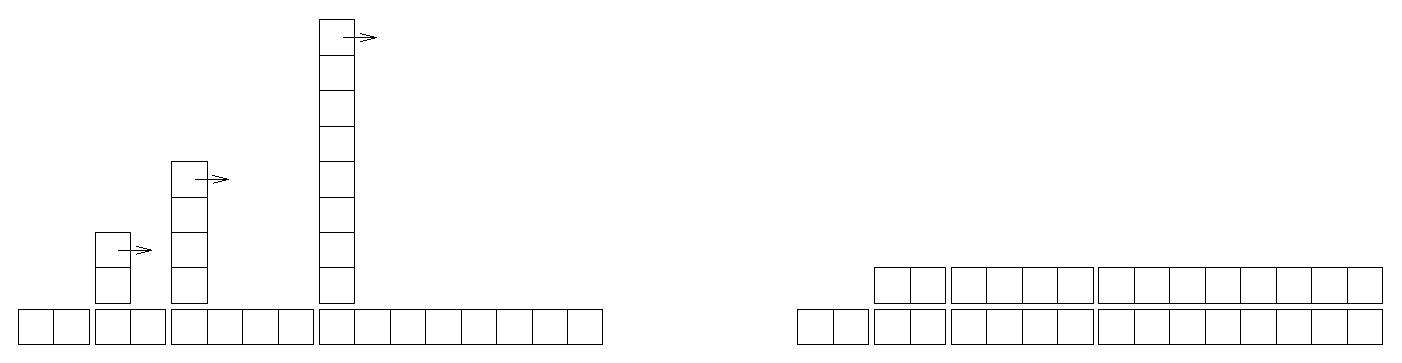
\includegraphics[width=5.5in]{figs/towers.eps}}
\afterfig

The extra work of rehashing appears as a sequence of increasingly
tall towers with increasing space between them.  Now if you knock
over the towers, amortizing the cost of resizing over all
adds, you can see graphically that the total cost after $n$
adds is $2n - 2$.

An important feature of this algorithm is that when we resize the
HashTable it grows geometrically; that is, we multiply the size by a
constant.  If you increase the size
arithmetically---adding a fixed number each time---the average time
per {\tt add} is linear.

You can download my implementation of HashMap from
\url{thinkcomplex.com/Map.py}, but remember that there 
is no reason to use it; if you want a map, just use a Python dictionary.

\begin{ex}

My implementation of {\tt HashMap} accesses the attributes of
{\tt BetterMap} directly, which shows poor object-oriented design.

Improve it by:

\begin{enumerate}

\item The special method \verb"__len__" is invoked by the built-in
function {\tt len}.  Write a \verb"__len__" method for {\tt BetterMap}
and use it in {\tt add}.

\item Use a generator to write {\tt BetterMap.iteritems}, and use it
in {\tt resize}.

\end{enumerate}

\end{ex}


\begin{ex}

Write an implementation of the dictionary interface called
{\tt TreeMap} that uses a red-black tree to perform {\tt add}
and {\tt get} in log time.

\end{ex}



\section{Summing lists}

Suppose you have a bunch of lists and you want to join them up
into a single list.  There are three ways you might do that
in Python:

\begin{itemize}

\item You could use the {\tt +=} operator:

\begin{verbatim}
    total = []
    for x in t:
        total += x
\end{verbatim}

\item Or the {\tt extend} method:

\begin{verbatim}
    total = []
    for x in t:
        total.extend(x)
\end{verbatim}

\item Or the built-in function {\tt sum}:

\begin{verbatim}
    total = sum(t, [])
\end{verbatim}

The second argument to {\tt sum} is the initial value for the total.

\end{itemize}

Without knowing how {\tt +=} and {\tt extend} and {\tt sum} are
implemented, it is hard to analyze their performance.  For example,
if {\tt total += x} creates a new list every time, the loop
is quadratic; but if it modifies {\tt total}, it's linear.

To find out, we could read the source code, but as an exercise, let's see
if we can figure it out by measuring run times.

A simple way to measure the run time of a program is to use
the function {\tt times} in the {\tt os} module, which returns
a tuple of floats indicating the time your process has used
(see the documentation for details).  I use a function {\tt etime},
which returns the sum of ``user time'' and ``system time'' which
is usually what we care about for performance measurement:

\begin{verbatim}
import os

def etime():
    """See how much user and system time this process has used
    so far and return the sum."""

    user, sys, chuser, chsys, real = os.times()
    return user+sys
\end{verbatim}

To measure the elapsed time of a function you can call
{\tt etime} twice and compute the difference:

\begin{verbatim}
    start = etime()

    # put the code you want to measure here

    end = etime()
    elapsed = end - start
\end{verbatim}

Alternatively, if you use IPython, you can use the
{\tt timeit} command. See \url{ipython.scipy.org}.

If an algorithm is quadratic, we expect the run time, $t$
as a function of input size, $n$, to look like this:

\[ t = a n^2 + b n + c \]

Where $a$, $b$ and $c$ are unknown coefficients.  If you take
the log of both sides you get:

\[ \log t \sim \log a + 2 \log n \]

For large values of $n$, the non-leading terms are insignificant
and this approximation is pretty good.  So if we plot $t$
versus $n$ on a log-log scale, we expect a straight line
with slope 2.

Similarly if the algorithm is linear, we expect a line with
slope 1.

I wrote three functions that concatenate lists: \verb"sum_plus" uses
{\tt +=}; \verb"sum_extend" uses {\tt list.extend}; and \verb"sum_sum"
uses {\tt sum}.  I timed them for a range of {\tt n} and plotted the
results on a log-log scale.  Figures~\ref{listsum1} and \ref{listsum2} show the
results.

\begin{figure}
\label{listsum1}
\centerline{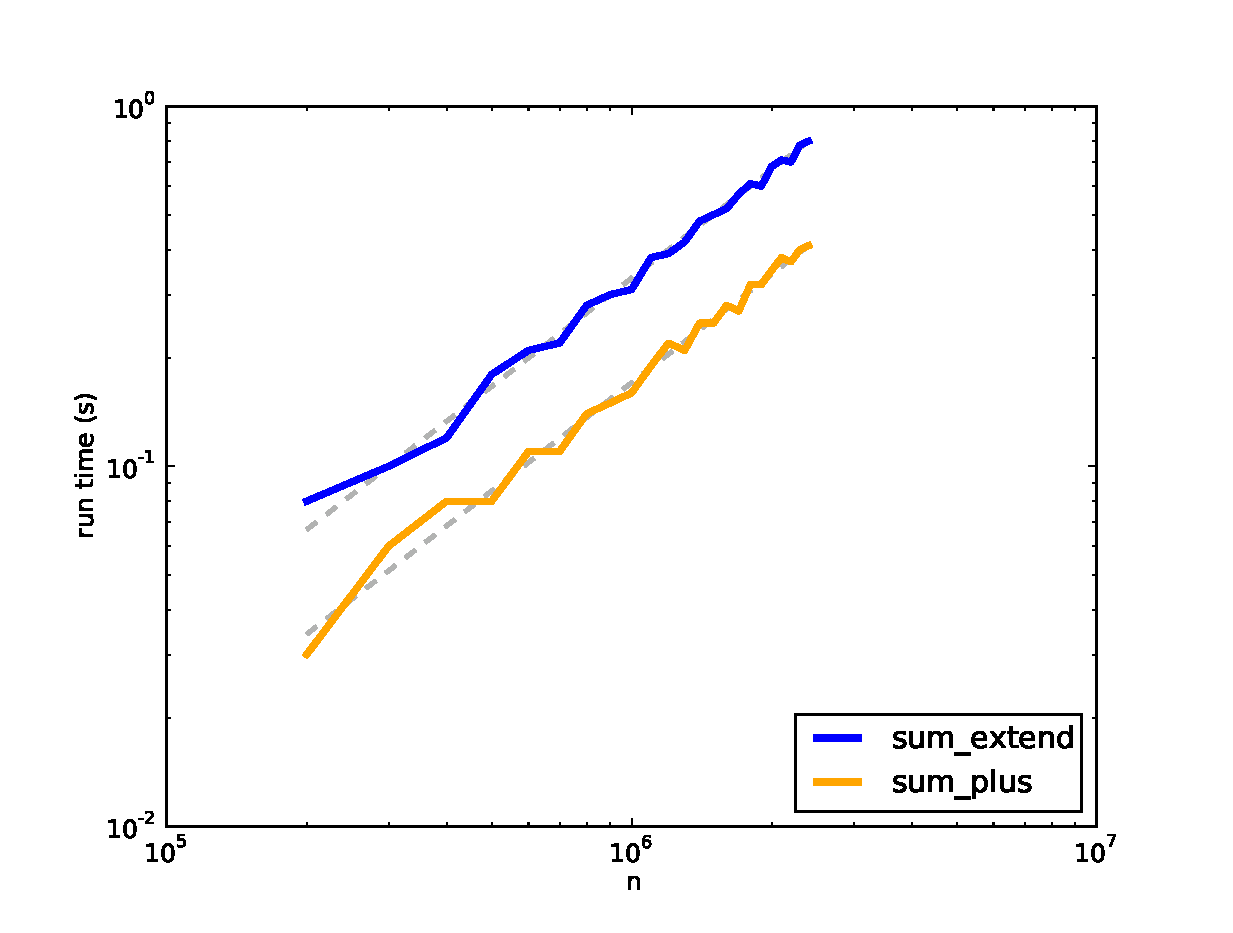
\includegraphics[height=2.5in]{figs/listsum1.eps}}
\caption{Runtime versus {\tt n}.  The gray lines have slope 1.}
\end{figure}

\begin{figure}
\label{listsum2}
\centerline{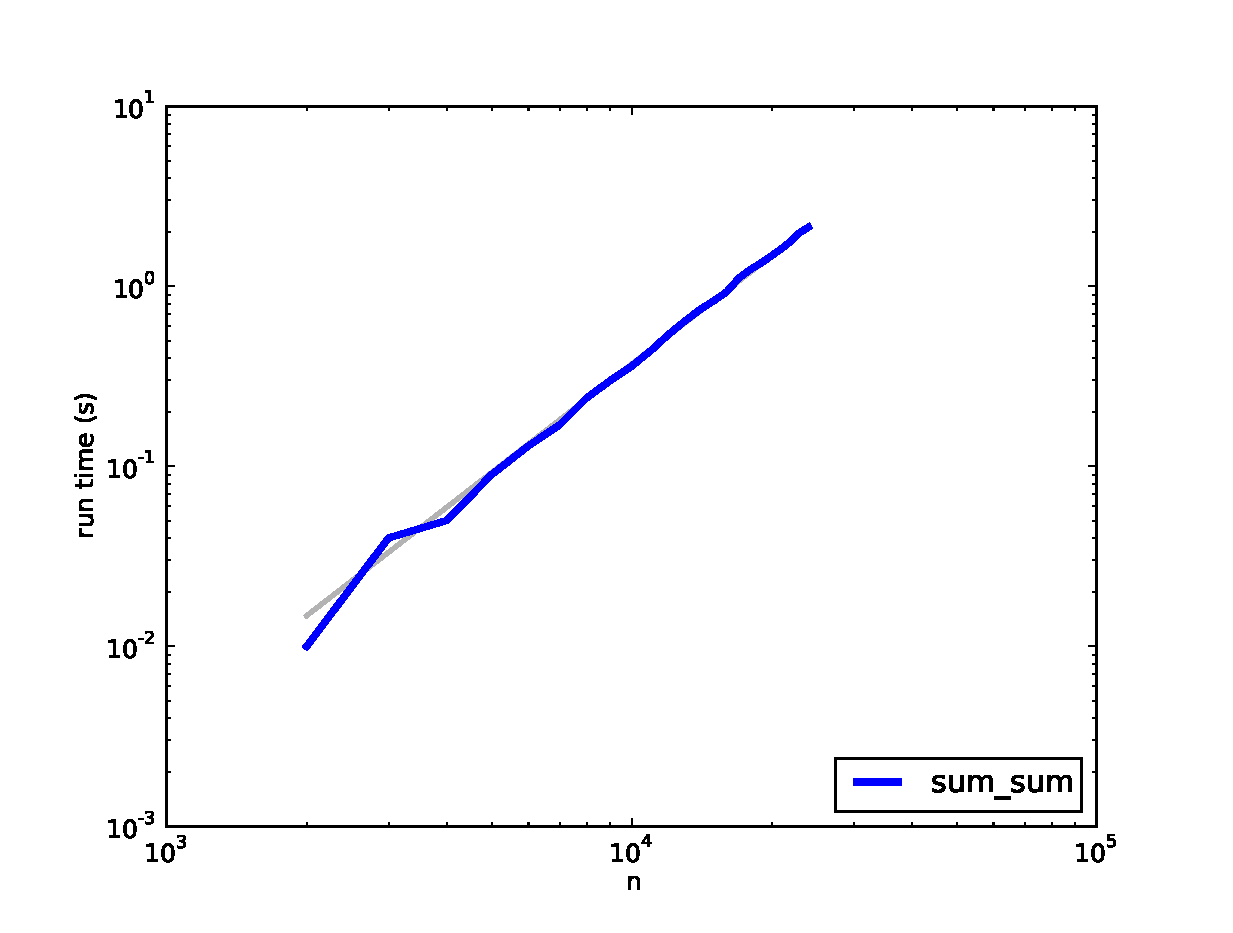
\includegraphics[height=2.5in]{figs/listsum2.eps}}
\caption{Runtime versus {\tt n}.  The gray line has slope 2.}
\end{figure}

In Figure~\ref{listsum1} I fit a line with slope 1 to the curves.
The data fit this line well, so we conclude
that these implementations are linear.  The implementation for {\tt +=}
is faster by a constant factor, probably because it takes some time
to look up the {\tt extend} method each time through the loop.

In Figure~\ref{listsum2} the data fit a line with slope 2, so the
implementation of {\tt sum} is quadratic.


\begin{ex}

Perform a similar experiment to test the performance of
{\tt LinearMap}, {\tt BetterMap} and {\tt HashMap}.

You can download my map implementations from
\url{thinkcomplex.com/Map.py}, and the code I used in this section
from \url{thinkcomplex.com/listsum.py}.

You will have to find a range
of {\tt n} that is big enough to show asymptotic behavior, but small
enough to run quickly.

\end{ex}


\section{List comprehensions}

One of the most common programming patterns is to traverse
a list while building a new list.

Here is an example that computes the square of each element in
a list accumulates the results:

\begin{verbatim}
    res = []
    for x in t:
        res.append(x**2)
\end{verbatim}

This pattern is so common that Python provides a more
concise syntax for it, called a {\bf list comprehension}.
In this context, the sense of ``comprehend'' is something
  like ``contain'' rather than ``understand.''  See
  \url{wikipedia.org/wiki/List_comprehension}.

Here's what it looks like:

\begin{verbatim}
    res = [x**2 for x in t]
\end{verbatim}

This expression yields the same result as the previous loop.  List
comprehensions tend to be fast because the loop is executed in C
rather than Python.  The drawback is that they are harder to debug.

List comprehensions can include an {\tt if} clause that selects a
subset of the items.  The following example makes a
list of the positive elements in {\tt t}:

\begin{verbatim}
    res = [x for x in t if x > 0]
\end{verbatim}

The following is a common idiom for making a list of tuples, where
each tuple is a value and a key from a dictionary:

\begin{verbatim}
    res = [(v, k) for k, v in d.iteritems()]
\end{verbatim}

In this case it is safe to use
{\tt iteritems}, rather than {\tt items}, because
the loop does not modify the dictionary; and it is likely to be
faster because it doesn't have to make a list, just an iterator.

It is also possible to nest {\tt for} loops inside
a list comprehension.  The following example builds a list
of Edges between each pair of vertices in {\tt vs}:

\begin{verbatim}
    edges = [Edge(v, w) for v in vs for w in vs if v is not w]
\end{verbatim}

Now that's pretty concise!

\begin{ex}

Review the methods your wrote in {\tt Graph.py} and see if any
can be rewritten using list comprehensions.

\end{ex}


\chapter{Small world graphs}

\section{Analysis of graph algorithms}

The order of growth for a graph algorithm is usually expressed
as a function of $|V|$, the number of vertices, and $|E|$, the number
of edges.

The order of growth for BFS is $O(|V| + |E|)$, which is a convenient
way to say that the run time grows in proportion to either $|V|$ or
$|E|$, whichever is ``bigger.''

To see why, think about these four operations: 

\begin{description}

\item Adding a vertex to the queue: this happens once for each
vertex, so the total cost is in $O(|V|)$.

\item Removing a vertex from the queue: this happens once for each
vertex, so the total cost is in $O(|V|)$.

\item Marking a vertex ``visited'': this happens once for each
vertex, so the total cost is in $O(|V|)$.

\item Checking whether a vertex is marked: this happens once each
edge, so the total cost is in $O(|E|)$.

\end{description}

Adding them up, we get $O(|V| + |E|)$.  If we know the relationship
between $|V|$ and $|E|$, we can simplify this expression.  For
example, in a regular graph, the number of edges is in $O(|V|)$ so BFS
is linear in $|V|$.  In a complete graph, the number of edges is in
$O(|V|^2)$ so BFS is quadratic in $|V|$.

Of course, this analysis is based on the assumption that all four
operations---adding and removing vertices, marking and checking
marks---are constant time.

Marking vertices is easy.  You can add an attribute to the {\tt
  Vertex} objects or use a dictionary\footnote{Or a set.  See
  \url{docs.python.org/lib/types-set.html}.} and the {\tt in} operator
to keep track of marked vertices.

But making a first-in-first-out (FIFO) queue that can add and remove
vertices in constant time turns out to be non-trivial.


\section{FIFO implementation}

A FIFO is a data structure that provides the following operations:

\begin{description}

\item[append:] Add a new item to the end of the queue.

\item[pop:] Remove and return the item at the front of the queue.

\end{description}

There are several good implementations of this data structure.
One is the {\bf doubly-linked list}, which 
you can read about at \url{wikipedia.org/wiki/Doubly-linked_list}.
Another is a circular buffer, which you can read about at
\url{wikipedia.org/wiki/Circular_buffer}.

\begin{ex}

Write an implementation of a FIFO using either a doubly-linked
list or a circular buffer.

\end{ex}

Yet another possibility is to use a Python dictionary augmented with
two indices: {\tt nextin} keeps track of the back of the queue; {\tt
  nextout} keeps track of the front.  Here is an
implementation\footnote{Based on a recipe in Martelli and Ascher, {\em
    Python Cookbook}, O'Reilly 2002}:

\begin{verbatim}
class DictQueue(dict):
    def __init__(self):
        self.nextin = 0
        self.nextout = 0

    def append(self, item):
        self.nextin += 1
        self[self.nextin] = item

    def pop(self):
        self.nextout += 1
        return dict.pop(self, self.nextout)
\end{verbatim}

{\tt append} increments {\tt nextin} and then stores the new item
in the dictionary; both operations are constant time\footnote{
When the index exceeds the capacity of an {\tt int}, Python
switches to {\tt long}.  After that, the increment and hash operations
are proportional to the number of digits in the index, which is
logarithmic in the number of items that have been added.}.

{\tt pop} increments {\tt nextout} and then uses {\tt dict.pop}
to remove and return the item at the end of the queue.  Again,
both operations are constant time.

As an alternative,
the Python {\tt collections} module provides an object called a {\tt
  deque}, which stands for ``double-ended queue''.  It is supposed to
be pronounced ``deck,'' but many people say ``deek.''  A Python deque
can be adapted very easily to implement a FIFO.

You can read about deques at \url{wikipedia.org/wiki/Deque}
and get the details of the Python implementation at
\url{docs.python.org/lib/deque-objects.html}.


\begin{ex}

The following implementation of a BFS\footnote{This was the
  implementation at \url{wikipedia.org/wiki/Breadth-first_search}
  before I fixed it.}  contains two performance errors.  What are
they?  What is the actual order of growth for this algorithm?

\begin{verbatim}
def bfs(top_node, visit):
    """Breadth-first search on a graph, starting at top_node."""
    visited = set()
    queue = [top_node]
    while len(queue):
        curr_node = queue.pop(0)    # Dequeue
        visit(curr_node)            # Visit the node
        visited.add(curr_node)
        # Enqueue non-visited and non-enqueued children
        queue.extend(c for c in curr_node.children
                     if c not in visited and c not in queue)
\end{verbatim}

\end{ex}


\section{Stanley Milgram}

Stanley Milgram was an American social psychologist who conducted
two of the most famous experiments in social science, the
Milgram experiment, which studied people's obedience to authority
(\url{wikipedia.org/wiki/Milgram_experiment})
and the Small World Experiment
\url{wikipedia.org/wiki/Small_world_phenomenon}, which studied
the structure of social networks.

In the Small World Experiment, Milgram sent a package to a number of
randomly-chosen people in Wichita, Kansas, with instructions asking
them to forward an enclosed letter to a target person, identified by
name and occupation, in Sharon, Massachusetts (which is the town near
Boston where I grew up).  The subjects were told that they could mail
the letter directly to the target person only if they knew him
personally; otherwise they were instructed to send it, and the same
instructions, to a relative or friend they thought would be more
likely to know the target person.

Many of the letters were never delivered, but of the ones that
were it turned out that the average path length---the number of
times the letters were forwarded---was about six.  This result
was taken to confirm previous observations (and speculations) that
the typical distance between any two people in a social network
is about ``six degrees of separation.''

This conclusion is surprising because most people expect social
networks to be localized---people tend to live near their
friends---and in a graph with local connections, path lengths tend to
increase in proportion to geographical distance.  For example, most of
my friends live nearby, so I would guess that the average distance
between nodes in a social network is about 50 miles.  Wichita is about
1600 miles from Boston, so if Milgram's letters traversed typical
links in the social network, they should have taken 32 hops, not six.


\section{Watts and Strogatz}

In 1998 Duncan Watts and Steven Strogatz published a paper
in {\em Nature}, ``Collective dynamics of 'small-world' networks,''
that proposed an explanation for the small world phenomenon.

Watts and Strogatz started with two kinds of graph that were well
understood: random graphs and regular graphs.  They looked at two
properties of these graphs, clustering and path length.

\begin{description}

\item Clustering is a measure of the ``cliquishness'' of the graph.
In a graph, a {\bf clique} is a subset of nodes that are
all connected to each other; in a social network, a clique is
a set of friends who all know each other.  Watts and Strogatz
defined a clustering coefficient that quantifies the likelihood
that two nodes that are connected to the same node are also
connected to each other.

\item Path length is a measure of the average distance between
two nodes, which corresponds to the degrees of separation in
a social network.

\end{description}

Their initial result was what you might expect: regular graphs
have high clustering and high path lengths;
random graphs with the same size tend to have low clustering
and low path lengths.  So neither of these is a good model of
social networks, which seem to combine high clustering with
short path lengths.

Their goal was to create a {\bf generative model} of a social
network.  A generative model tries to explain a phenomenon by
modeling a process that builds or leads to the phenomenon.  In
this case Watts and Strogatz proposed a process for building
small-world graphs:

\begin{enumerate}

\item Start with a regular graph with $n$ nodes and degree $k$.

\item Choose a subset of the edges in the graph and ``rewire''
them by replacing them with random edges.

\end{enumerate}

The proportion of edges that are rewired is a parameter, $p$,
that controls how random the graph is.  With $p=0$, the graph
is regular; with $p=1$ it is random.

Watts and Strogatz found that small values of $p$ yield graphs
with high clustering, like a regular graph, and low path
lengths, like a random graph.

\begin{ex}

Read the Watts and Strogatz paper and answer the following
questions:

\begin{enumerate}

\item What process do Watts and Strogatz use to rewire their
graphs?

\item What is the definition of the clustering coefficient $C(p)$?

\item What is the definition of the average path length $L(p)$?

\item What real-world graphs did Watts and Strogatz look at?
What evidence do they present that these graphs have the
same structure as the graphs generated by their model?

\end{enumerate}

\end{ex}  


\begin{ex}

Create a file named {\tt SmallWorldGraph.py} and define a class named 
{\tt SmallWorldGraph} that inherits from {\tt RandomGraph}.

\begin{enumerate}

\item Write a method called {\tt rewire} that takes a probability {\tt
  p} as a parameter and, starting with a regular graph, rewires
the graph using Watts and Strogatz's algorithm.

\item Write a method called \verb"clustering_coefficient" that
computes and returns the clustering coefficient as defined in the
paper.

\item Make a graph that replicates the line marked $C(p)/C(0)$ in
Figure 2 of the paper.  In other words, 
confirm that the clustering coefficient drops off slowly for
small values of $p$.

\end{enumerate}

Before we can replicate the other line, we have to learn about shortest
path algorithms.

\end{ex}


\section{Dijkstra}

Edsger W. Dijkstra was a Dutch computer scientist who invented an
efficient shortest-path algorithm (see
\url{wikipedia.org/wiki/Dijkstra's_algorithm}), He also invented the
semaphore, which is a data structure used to coordinate programs that
communicate with each other (see
\url{wikipedia.org/wiki/Semaphore_(programming)} and Downey, {\em The
  Little Book of Semaphores}).

Dijkstra is also famous (and notorious) as the author of a series
of essays on computer science.
Some, like ``A Case against the GO TO Statement,'' have
had a profound effect on programming practice.
Others, like
``The Cruelty of Really Teaching Computing Science,'' are
entertaining in their cantankerousness, but less effective.

Dijkstra's algorithm solves the ``single source shortest path problem,''
which means that it finds the minimum distance from a given ``source''
node to every other node in the graph (or at least every connected
node).

We will start with a simplified version of the algorithm that
considers all edges the same length.  The more general version
works with any non-negative edge lengths.

The simplified version is similar to the breadth-first search
in Section~\ref{bfs} except that instead of marking visited nodes,
we label them with their distance from the source.  Initially
all nodes are labeled with an infinite distance.  Like a
breadth-first search, Dijkstra's algorithm uses a queue of
discovered unvisited nodes.

\begin{enumerate}

\item Label the source node with distance 0 and add it to the queue.

\item Remove a vertex from the queue and call its distance $d$.  Find
  the vertices it is connected to.  For each connected vertex still
  labeled with distance infinity, replace the distance with $d+1$ and
  add it to the queue.

\item If the queue is not empty, go back to Step 2.

\end{enumerate}

The first time you execute Step 2, the only node in the queue
has distance 0.  The second time, the queue contains all
nodes with distance 1.  Once those nodes are processed, the
queue contains all nodes with distance 2, and so on.

So when a node is discovered for the first time, it is labelled
with the distance $d+1$, which is the shortest path to that
node.  It is not possible that you will discover a shorter
path later, because if there were a shorter path, you would
have discovered it sooner.  Of course, that is not a proof
of the correctness of the algorithm, but it is a sketch of
the structure of the proof, which is by contradiction.

In the more general case, where the edges have different lengths,
it is possible to discover a shorter path after you have
discovered a longer path, so a little more work is required.

\begin{ex}

Write an implementation of Dijkstra's algorithm and use it
to compute the average path length of a SmallWorldGraph.

Make a graph that replicates the line marked $L(p)/L(0)$ in
Figure 2 of the Watts and Strogatz paper.  Confirm that the 
average path length drops off quickly for
small values of $p$.  What is the range of values for $p$
that yield graphs with high clustering and low path lengths?

\end{ex}


\begin{ex}

A natural question about the Watts and Strogatz paper is
whether the small world phenomenon is specific to their
generative model or whether other similar models yield
the same qualitative result (high clustering and low path lengths).

To answer this question, choose a variation of the
Watts and Strogatz model and replicate their Figure 2.
There are two kinds of variation you might consider:

\begin{itemize}

\item Instead of starting with a regular graph, start with
another graph with high clustering.  One option is a locally-connected
graph where vertices are placed at random locations in the plane
and each vertex is connected to its nearest $k$ neighbors.

\item Experiment with different kinds of rewiring.

\end{itemize}

If a range of similar models yield similar behavior, we
would say that the results of the paper are {\bf robust}.

\end{ex}


\begin{ex}

To compute the average path length in a SmallWorldGraph, you
probably ran Dijkstra's single-source shortest path algorithm
for each node in the graph.  In effect, you solved the
``all-pairs shortest path'' problem, which finds the shortest path
between all pairs of nodes.

\begin{enumerate}

\item Find an algorithm for the all-pairs shortest path problem
and implement it.  Compare the run time with your
``all-source Dijkstra'' algorithm.

\item Which algorithm gives better order-of-growth run time
as a function of the number of vertices and edges?  Why do you
think Dijkstra's algorithm does better than the order-of-growth
analysis suggests?

\end{enumerate}

\end{ex}

\section{What kind of explanation is {\em that}?}

If you asked me why planetary orbits are approximately elliptical,
I might start by modeling a planet and a star as point masses; I
would look up the law of universal gravitation at
\url{wikipedia.org/wiki/Newton's_law_of_universal_gravitation}
and use it to write a differential equation for the motion of
the planet.  Then I would either derive the orbit equation or,
more likely, look it up at \url{wikipedia.org/wiki/Orbit_equation}.
With a little algebra, I could derive the conditions that
yield an elliptical orbit.  Then I would argue that the objects
we consider planets satisfy these conditions.

People, or at least scientists, are generally satisfied with
this kind of explanation.  One of the reasons for its appeal
is that the assumptions and approximations in the model seem
reasonable.  Planets and stars are not really point masses,
but the distances between them are so big that their actual
sizes are negligible.  Planets in the same solar system can
affect each others' orbits, but the effect is usually small.
And we ignore relativistic effects, again on the assumption that
they are small.

This explanation is also appealing because it is equation-based.
We can express the orbit equation in a closed form, which means
that we can compute orbits very efficiently.  It also means that
we can derive general expressions for the orbital velocity,
orbital period, and other quantities.

Finally, I think this kind of explanation is appealing because
it has the form of a mathematical proof.  It starts from a
set of axioms and derives the result by logic and analysis.
But it is important to remember that the proof pertains to the
model and not the real world.  That is, we can prove that
an idealized model of a planet yields an elliptic orbit, but
we can't prove that the model pertains to actual planets (in
fact, it does not).

By comparison, Watts and Strogatz's explanation of the small
world phenomenon may seem less satisfying.  First, the model
is more abstract, which is to say less realistic.  Second,
the results are generated by simulation, not by mathematical
analysis.  Finally, the results seem less like a proof and
more like an example.

Many of the models in this book are like the Watts and
Strogatz model: abstract, simulation-based and (at least
superficially) less formal than conventional mathematical 
models.  One of the goals of this book it to consider the
questions these models raise:

\begin{itemize}

\item What kind of work can these models do: are they predictive, or
  explanatory, or both?

\item Are the explanations these models offer less satisfying than
  explanations based on more traditional models?  Why?

\item How should we characterize the differences between these and
  more conventional models?  Are they different in kind or only in
  degree?

\end{itemize}

Over the course of the book I will offer my answers
to these questions, but they are tentative and sometimes
speculative.  I encourage you to consider them skeptically
and reach your own conclusions.





\chapter{Scale-free networks}

\section{Zipf's Law}

Zipf's law describes a relationship between the frequencies and ranks
of words in natural languages\footnote{See
  \url{wikipedia.org/wiki/Zipf's_law}}.  The ``frequency'' of
a word is the number of times it appears in a body of work.
The ``rank'' of a word is its position in a list of words
sorted by frequency: the most common word has rank 1, the
second most common has rank 2, etc.

Specifically, Zipf's Law
predicts that the frequency, $f$, of the word with rank $r$ is:

\[ f = c r^{-s} \]
%
where $s$ and $c$ are parameters that depend on the language and the
text.

If you take the logarithm of both sides of this equation, you get:

\index{logarithm}

\[ \log f = \log c - s \log r \]
%
So if you plot $\log f$ versus $\log r$, you should get
a straight line with slope $-s$ and intercept $\log c$.

\begin{ex}
Write a program that reads a text from a file, counts word
frequencies, and prints one line for each word, in descending order of
frequency.  You can test it by downloading an out-of-copyright book in
plain text format from {\tt gutenberg.net}.  You might want to remove
punctuation from the words.

If you need some help getting started, you can download
\url{thinkcomplex.com/Hist.py}, which provides an
object named {\tt Hist} that you might find useful.

Plot the results and check whether they form
a straight line.  Can you estimate the value of $s$?

You might want to use the {\tt pylab}
package, which provides easy-to-use functions to generate
a variety of plots.  In particular, {\tt pylab.loglog} plots
a series of points on a log-log scale.  {\tt pylab} is part of
a larger package called {\tt matplotlib}; it is
not included in all Python distributions, so you might have to
install it.

Here is an example that generates a simple graph:

\begin{verbatim}
import pylab

# compute lists of x and y values
xs = range(0, 10)
ys = [x**2 for x in xs]

# plot the data
pylab.plot(xs, ys, '-ro')

# set title and labels
pylab.title('Parabola')
pylab.xlabel('x')
pylab.ylabel('y = x**2')

# show the plot
pylab.show()
\end{verbatim}

{\tt pylab.plot} takes two lists as parameters.  If you have a list of
pairs instead, you can use {\tt zip} and the scatter operator to
``transpose'' it.  For example, if {\tt t} is a list of pairs, {\tt
  zip(*t)} returns a pair of lists.

The most common gotcha with {\tt pylab} is that you have to
call {\tt pylab.show} to see the plot.  You can read more
about it at \url{matplotlib.sourceforge.net}.

You can download my solution from
\url{thinkcomplex.com/Zipf.py}

\end{ex}



\section{Cumulative distributions}

A distribution is a statistical description of a set of values.
For example, if you collect the population of every city and town
in the U.S., you would have a set of about 14,000 integers.

The simplest description of this set is a list of numbers, which
would be complete but not very informative.  A more concise description
would be a statistical summary like the mean and variation, but
that is not a complete description because there are many sets
of values with the same summary statistics.

One alternative is a histogram, which divides the range of
possible values into ``bins'' and counts the number of values that
fall in each bin.  Histograms are common, so they are
easy to understand, but they have some drawbacks: the primary
one is that it is tricky to get the bin size right.  If the bins
are too small, then the number of values in each bin is also small,
so the histogram doesn't give much insight.  If the bins are
too large, they lump together a wide range of values, which
obscures details that might be important.

A better alternative is a {\bf cumulative distribution}, which shows
the percentage of values less than or equal to $x$ for a range of
$x$ that sweeps from the smallest value in the set to the
highest.

For example, the following figure shows the cumulative distribution
function (CDF), for the values $(1,2,2,4,5)$.

\beforefig
\centerline{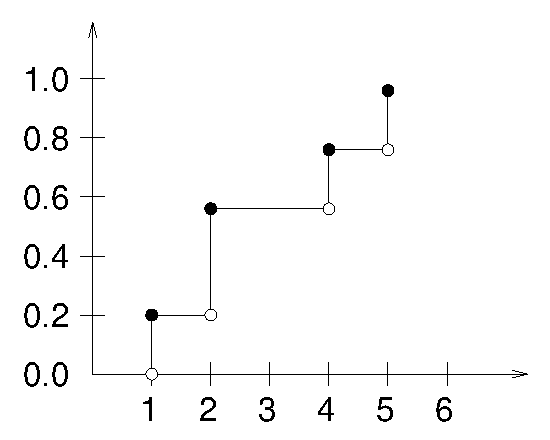
\includegraphics[width=2.5in]{figs/cdf.eps}}
\afterfig

The range of the CDF is always from 0 to 1.  The values on the
$y$-axis are sometimes called {\bf percentiles}, although
strictly-speaking the range of a percentile is from 0 to 100.  The
values on the $x$-axis are called {\bf quantities}, or sometimes
``quantiles.''

The filled and empty circles indicate the value
of the function at integral values: for example, $cdf(1) = 0.2$
because 20\% of the values in the set are less than or equal to 1.

\begin{ex}
Write a definition for a class named {\tt Dist} that provides the
following methods:

\begin{description}

\item[{\tt\_\_init\_\_}:] Takes a histogram object similar to
the one defined in \url{thinkcomplex.com/Hist.py}
and builds a representation of the distribution.

For example, to make a distribution of the values $(1,2,2,4,5)$
you would run:

\begin{verbatim}
h = Hist([1,2,2,4,5])
d = Dist(h)
\end{verbatim}

\item[percentile:] Takes a quantity and returns the corresponding
percentile.  For example, given the previous values, {\tt d.percentile(2)}
should return $0.6$.

\item[{\tt print\_cdf}:] Print the quantities in the distribution
and their corresponding percentiles, with two lines per
quantity.  For the previous distribution, the output should be:

\begin{verbatim}
1 0.0
1 0.2
2 0.2
2 0.6
4 0.6
4 0.8
5 0.8
5 1.0
\end{verbatim}

\item[{\tt plot\_cdf}:] Use {\tt pylab} to plot the distribution
in the style of the figure above.  You should plot two points
per quantity to make a stair-step pattern.  You don't have to
plot the filled and empty circles, but you can.


\end{description}

You should give some thought to choosing a data structure to
represent a distribution.  {\tt percentile} should be $O(\log n)$,
where $n$ is the
number of {\em unique} quantities in the distribution.
The other methods should be linear in $n$.

You can download my solution from
\url{thinkcomplex.com/Dist.py}

\end{ex}


\section{Closed-form distributions}

The distributions we have seen so far are sometimes called
{\bf empirical distributions} because they are based on a
dataset that comes from some kind of empirical observation.

An alternative is what I will call a {\bf closed-form distribution},
which is characterized by a CDF that can be expressed as a closed-form
function.  Some of these distributions, like the
Gaussian\footnote{This is not a perfect example, since the CDF of a
  Gaussian is an integral with no closed-form solution.} or normal
distribution, are well known, at least to people who have studied
statistics.  Many real world phenomena can be approximated by
closed-form distributions, which is why they are useful.

For example, if you observe a mass of radioactive material with
an instrument that can detect decay events, the distribution
of times between events will most likely fit an exponential
distribution.  The same is true for any series of events where
an event is equally likely at any time.

The CDF of the exponential distribution is:

\[ cdf(x) = 1 - e^{-\lambda x} \]

The parameter, $\lambda$, determines the mean and variance
of the distribution.  This equation can be used to derive
a simple visual test for whether a dataset can be well
approximated by an exponential distribution.  All you
have to do is plot the {\bf complementary distribution}
on a log-$y$ scale.

The complementary distribution (CCDF) is just $1 - cdf(x)$; 
if you plot the complementary distribution of a dataset
that you think is exponential, you expect to see a function
like:

\[ y = 1 - cdf(x) \sim e^{-\lambda x} \]

If you take the log of both sides of this equation, you get:

\[ \log y \sim -\lambda x \]

So on a log-$y$ scale the CCDF should look like a straight line
with slope $-\lambda$.

As an example, I will analyze the time of
birth for 44 babies born in a 24-hour period in a hospital in
Brisbane, Australia.\footnote{This example is based on information
  and data from Dunn, ``A Simple Dataset for Demonstrating Common
  Distributions,'' Journal of Statistics Education v.7, n.3 (1999).
You can download a file with this data from 
\url{thinkcomplex.com/babyboom.dat}.}.

Using the list of birth times, I computed the ``interarrival times;''
that is, the times between successive births.  The following figure
shows the CCDF of these values.  The graph on the right is on a
log-$y$ scale.  It is not particularly straight, which suggests that
the exponential model is only an approximation of the observed
process.  Most likely the underlying assumption---that a birth is
equally likely at any time of day---is not exactly true.

\beforefig
\centerline{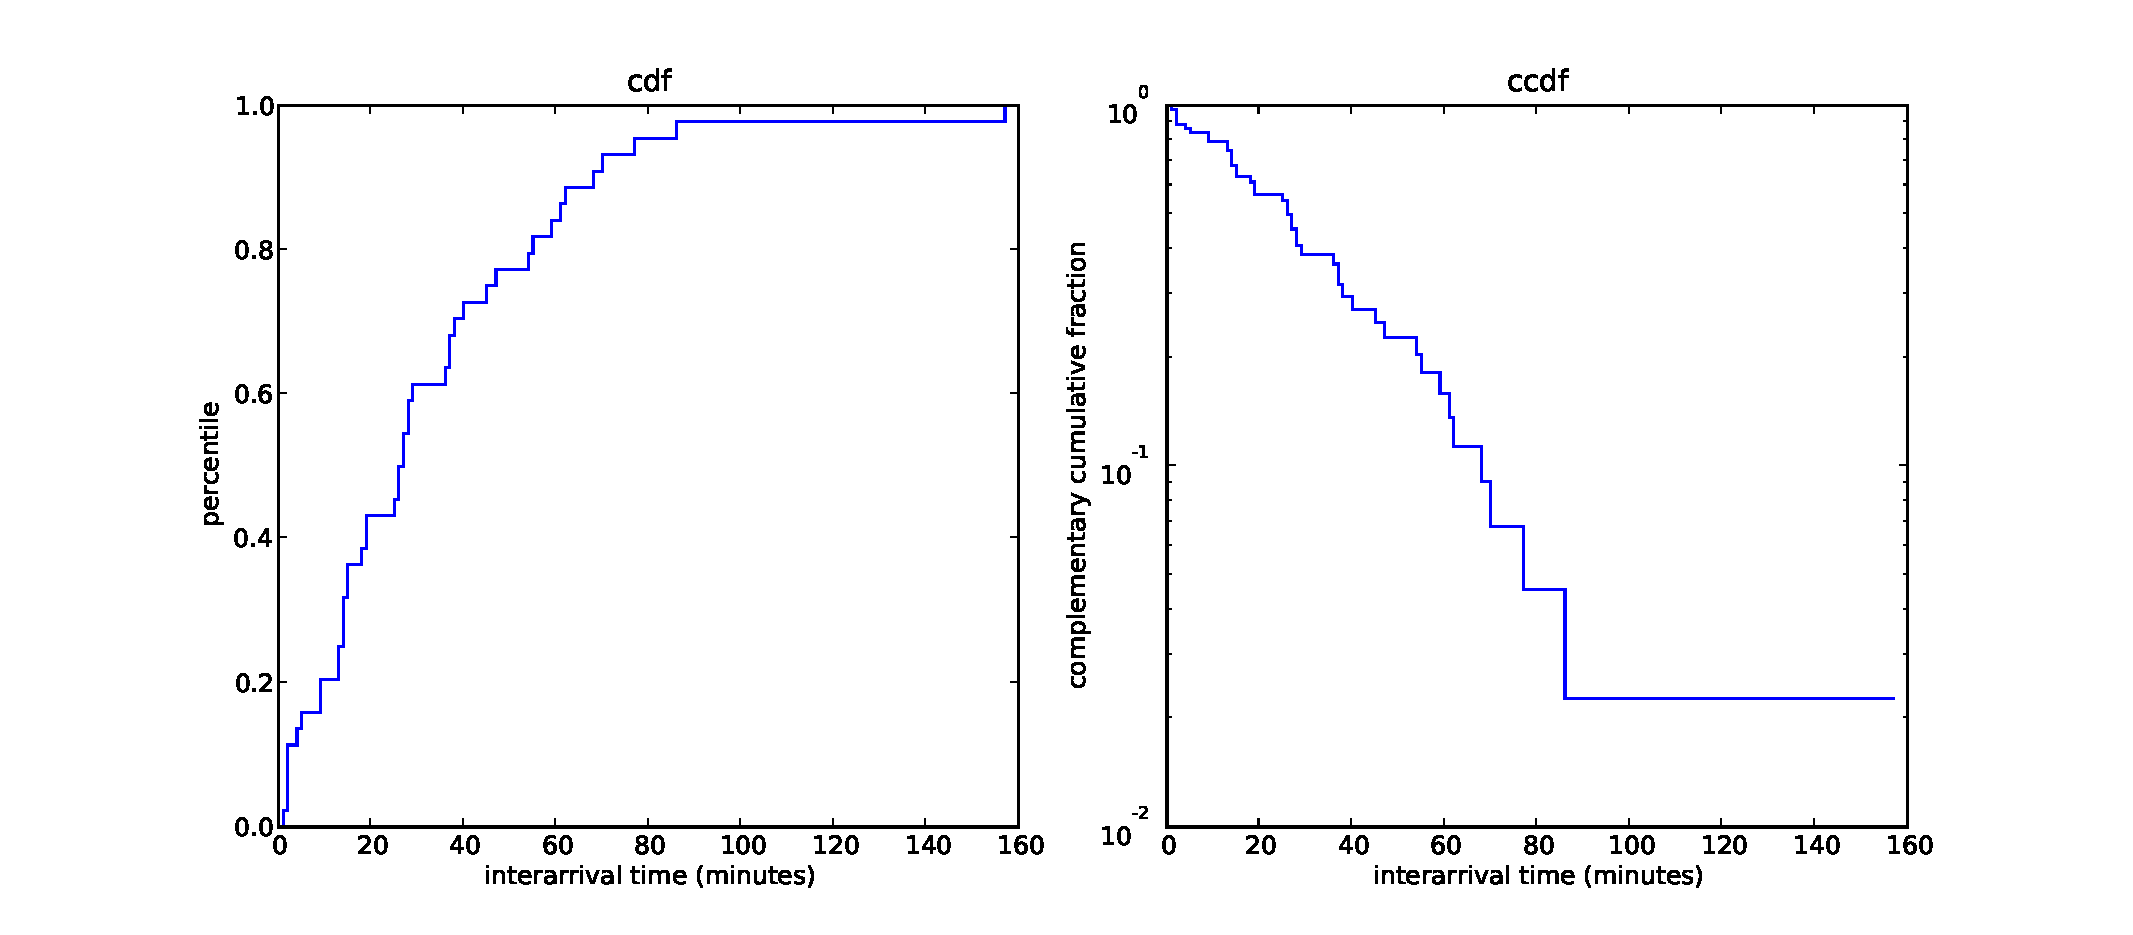
\includegraphics[width=5.5in]{figs/babyboom_cdf.eps}}
\afterfig

\begin{ex}
In your {\tt Dist} class, add
a method called \verb"plot_ccdf" that plots the complementary
CDF of the distribution.
\end{ex}

\begin{ex}
Use the function {\tt expovariate} in the {\tt random} module
to generate 44 values from an exponential distribution with
mean 32.6.  Plot the CCDF on linear and log-$y$ scales and compare
it to the figure above.  
\end{ex}


\section{Pareto distributions}

The Pareto distribution is named after the economist Vilfredo
Pareto, who used it to describe the distribution of wealth
(see \url{wikipedia.org/wiki/Pareto_distribution}).  Since then,
people have used it to describe
a variety of phenomena in the natural and social sciences,
including sizes of cities and towns, sand particles
and meteorites, forest fires and earthquakes.

The Pareto distribution is characterized by a CDF with the following
functional form:

\[ 1- \left( \frac{x}{x_m} \right) ^{-\alpha} \]

The parameters $x_m$ and $\alpha$ determine the location and shape of
the distribution.  $x_m$ is the minimum possibile quantity.

Values from a Pareto distribution often have these properties:

\begin{description}

\item[Long tail:] Pareto distributions contain many small values
and a few very large ones.  

\item[80/20 rule:] The large values in a Pareto distribution are
so large that they add up to a disproportionate share of the total.
In the context of wealth, the 80/20 rule says that 20\% of the
people own 80\% of the wealth.

\item[Scale free:] Short-tailed distributions are centered around
a typical size, which is called a ``scale.''  For example, the
great majority of adult humans are between 100 and 200 cm in height,
so we could say that the scale of human height is a few hundred
centimeters.  But for long-tailed distributions, there is no
similar range (bounded by a factor of two) that contains the
bulk of the distribution.  So we say that these distributions
are ``scale-free.''

\end{description}

To get a sense of the difference between the Pareto and Gaussian
distributions, imagine what the world would be like if the
distribution of human height were Pareto.  Using the same minimum
height, $x_m = 100$ cm, we could choose $\alpha = 1.7$, so that the median
height is about 150 cm.

Here are empirical CDFs for samples with $n=9000$ drawn 
from these two distributions:

\beforefig
\centerline{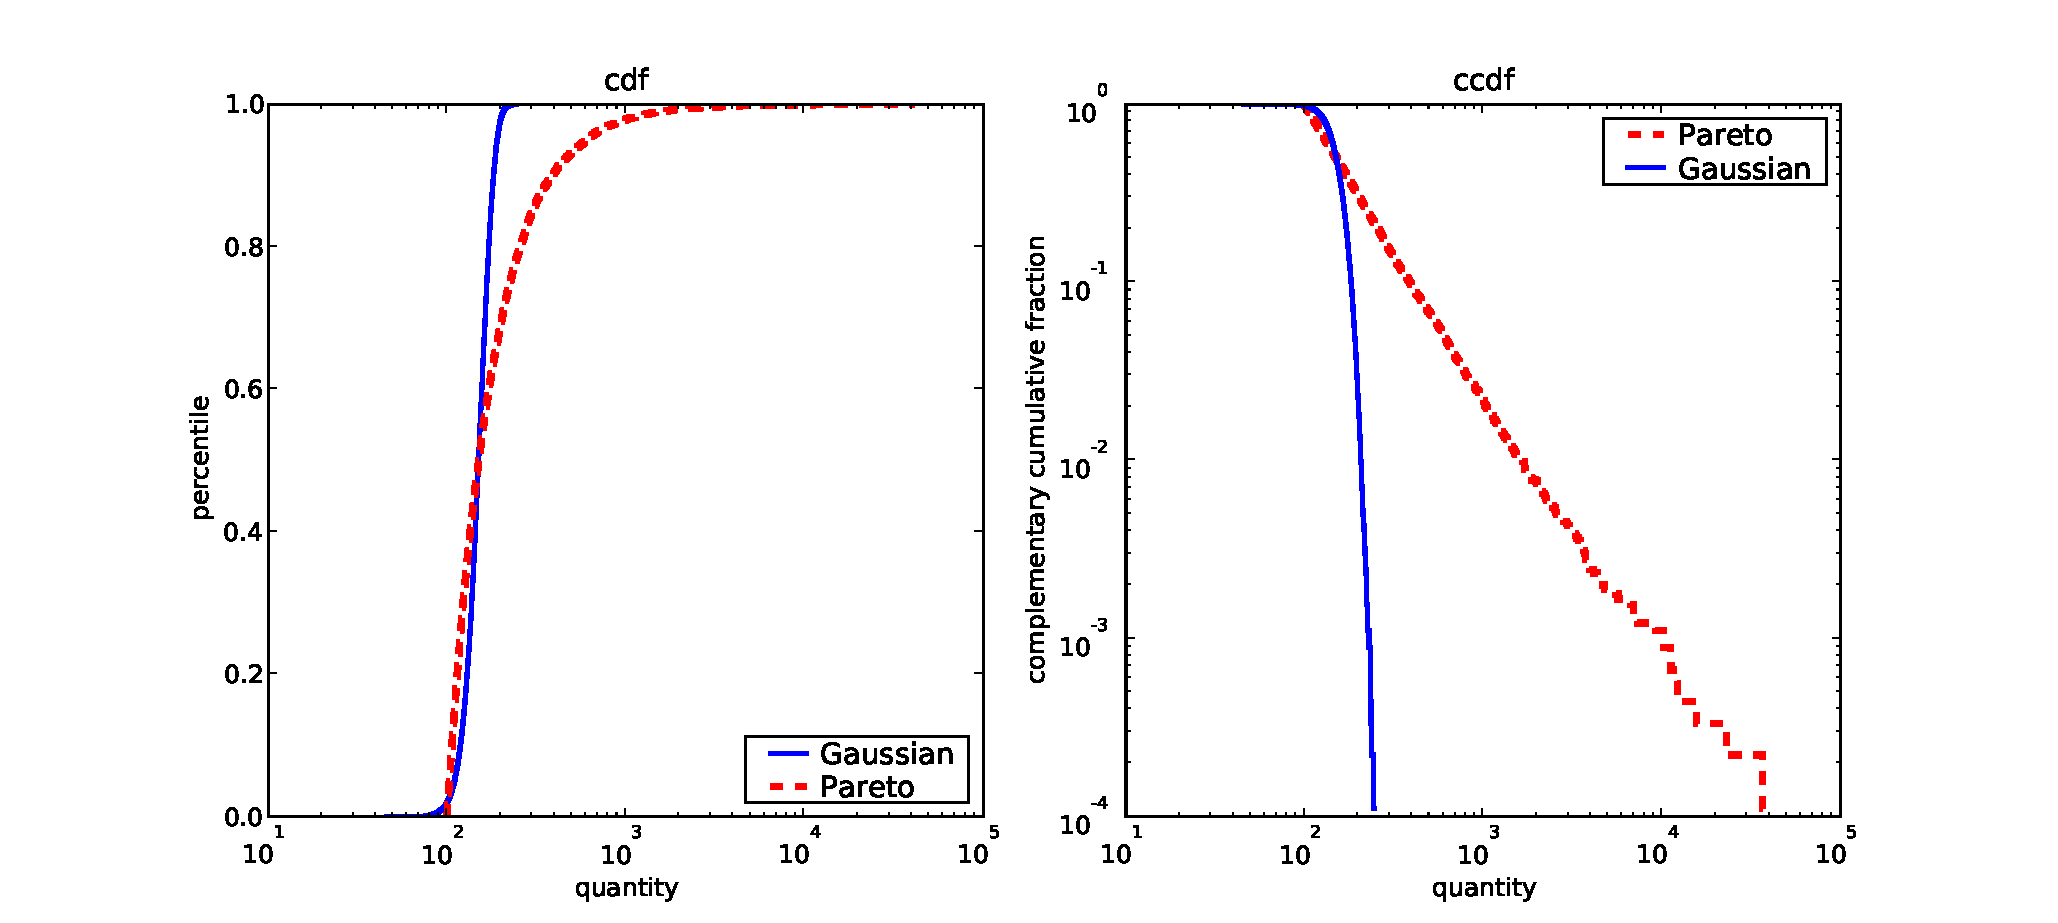
\includegraphics[width=5.5in]{figs/height_cdf.eps}}
\afterfig

The figure on the left is on a log-$x$ scale.  It shows that the
median and lower bounds of the distributions are the same, but
the Pareto distribution has a longer tail.  The figure on the
right is on a log-log scale.  The Pareto distribution is a straight
line except in the extreme tail, where it is noisy because of
the limitations of a finite sample.

If you generate 6 billion random values from the Gaussian distribution
shown in the figure, you would guess that the tallest person in the
world is about 255 cm.  In fact, the tallest currently living person,
Leonid Stadnyk, is 259 cm.

But if you generate 6 billion random values from the Pareto
distribution, you will see that the tallest person in the world could
easily be taller than 80.5 km, which would technically make him or her
an astronaut, at least in the United States (see
\url{wikipedia.org/wiki/Earth's_atmosphere}).  That's what it means to
be scale-free!

There is a simple visual test that can indicate whether an empirical
distribution is well-characterized by a Pareto distribution: on a
log-log scale, the CCDF looks like a straight line.  The derivation is
similar to what we saw in the previous section.

The equation for the CCDF is:

\[ y = 1 - cdf(x) \sim \left( \frac{x}{x_m} \right) ^{-\alpha} \]

Taking the log of both sides yields:

\[ \log y \sim -\alpha (\log x - \log x_m ) \]

So if you plot $\log y$ versus $\log x$, it should look like a
straight line with slope $-\alpha$ and intercept $-\alpha \log x_m$.

\begin{ex}

The Weibull distribution is a generalization of the exponential
distribution that comes up in failure analysis
(see \url{wikipedia.org/wiki/Weibull_distribution}).

Can you find a transformation that makes a Weibull distribution look
like a straight line?  What do the slope and intercept of the
line indicate?

Use {\tt random.weibullvariate} to generate a sample from a
Weibull distribution and use it to test your transformation.

\end{ex}


\begin{ex}
The distribution of populations for cities and towns has been proposed
as an example of a real-world phenomenon that can be described
with a Pareto distribution.

The U.S. Census Bureau publishes data on the population of every
incorporated city and town in the United States.  I have written a
small program that downloads this data and converts it into a
convenient form.  You can download it from
\url{thinkcomplex.com/populations.py}.  

\begin{enumerate}

\item Read over the program to make sure you know what it does and then
  write a program that computes and plots the distribution of
  populations for the 14593 cities and towns in the dataset.

\item In your {\tt Dist} class, write a function called {\tt quantile}
  that takes a percentile as a parameter and returns the corresponding
  quantity.  What is the median size in this distribution (the
  quantity that corresponds to the 50th percentile)?  What are the
  25th and 75th percentiles?

\item Plot the CDF on linear and log-$x$ scales so you can get a sense
  of the shape of the distribution.  Then plot the CCDF on a log-log
  scale to see if it has the characteristic shape of a Pareto
  distribution.

\item Use your plot to estimate values for the parameters $x_m$ and
  $\alpha$.  Then use the function {\tt paretovariate} in the {\tt random}
  module to generate 14593 values from a Pareto distribution with the
  parameters you estimated in the previous problem.  Plot the CCDF on
  a log-log scale and compare it the CCDF of the observed data.

\end{enumerate}

What conclusion do you draw about the distribution of sizes
for cities and towns?

\end{ex}

\newcommand{\Barabasi}{Barab\'{a}si}

\section{\Barabasi~ and Albert}

In 1999 \Barabasi~ and Albert published a paper in {\em Science},
``Emergence of Scaling in Random Networks,''
that characterizes the structure (also called ``topology'') of
several real-world networks, including graphs that represent
the interconnectivity of movie actors, world-wide web (WWW) pages,
and elements in the electrical power grid in the western
United States.  

They measure the degree (number of connections) of each node and
compute $P(k)$, the probability that a vertex has degree $k$; then
they plot $P(k)$ versus $k$ on a log-log scale.  The tail of the plot
fits a straight line, so they conclude that it obeys a {\bf power law}:
as $k$ gets large, $P(k)$ is asymptotic to $k^{- \gamma}$, where
$\gamma$ is a parameter that determines the rate of decay.

They also propose a model that generates random graphs with the same
property.  The essential features of the model, which distinguish it
from the \Erdos-\Renyi~ model and the Watts-Strogatz model, are:

\begin{description}

\item[Growth:]  Instead of starting with a fixed number of vertices,
\Barabasi~ and Albert start with a small graph, add vertices over
time, and characterize the structure of the graph as the number
of vertices grows.

\item[Preferential attachment:] When a new edge is created, it is
more likely to connect to a vertex that already has a large number
of edges.  This ``rich get richer'' effect is characteristic of
the growth patterns of some real-world networks.

\end{description}

Finally, they show that graphs generated by this model have a
distribution of degrees that obeys a power law.  Graphs that
have this property are sometimes called {\bf scale-free networks}
(see \url{wikipedia.org/wiki/Scale-free_network}),
but the name can be confusing because it is the distribution
of degrees that is scale-free.  

In order to maximize confusion, distributions that obey the power law
are also sometimes called {\bf scaling distributions} because they are
invariant under a change of scale.  That means that if you change the
units the quantities are expressed in, the slope parameter, $\gamma$,
doesn't change.  You can read \url{wikipedia.org/wiki/Power_law} for
the details, but it is not important for what we are doing here.


\begin{ex}

This exercise asks you to make connections between the Watts-Strogatz (WS)
and \Barabasi-Albert (BA) models:

\begin{enumerate}

\item Read \Barabasi~ and Albert's paper and implement their algorithm
for generating graphs.  See if you can replicate their Figure 2(A),
which shows $P(k)$ versus $k$ for a graph with 150 000 vertices.

\item Use the WS model to generate the largest graph you can in
a reasonable amount of time.  Plot $P(k)$ versus $k$ and see if
you can characterize the rate of decay.

\item Use the BA model to generate a graph with about 1000 vertices
and compute the characteristic length and clustering coefficient
as defines in the Watts and Strogatz paper.  Do scale-free networks
have the characteristics of a small-world graph?

\end{enumerate}

\end{ex}




\section{Zipf, Pareto and power laws}


At this point we have seen three phenomena that yield a straight line
on a log-log plot:

\begin{description}

\item[Zipf law:] A Zipf plot shows frequency as a function of rank. 

\item[Pareto CCDF:] A CCDF shows percentile as a function of quantile.

\item[Power law distribution:] A power law plot shows frequency
(or probability) as a function of quantile.

\end{description}

The similarity in these plots is not a coincidence; these
visual tests are closely related.

Starting with a power-law distribution, we have:

\[ P(k) \sim k^{- \gamma} \]

$P(k)$ is the probability that a random variable $X$ equals $k$,
so the cumulative distribution of $X$ is:

\[ cdf(x) = Pr\{X \le x \} = \sum_{k=0}^x P(k) \]

For large values of $k$ we can approximate the summation with
an integral:

\[ \sum_{k=0}^x k^{- \gamma} \sim \int_{k=0}^x k^{- \gamma} = 
\frac{1}{\gamma -1} (1 - x^{-\gamma + 1}) \]

To make this a proper CDF we could normalize it so that it
goes to 1 as $x$ goes to infinity, but that's not necessary,
because all we need to know is:

\[ cdf(x) \sim 1 - x^{-\gamma + 1} \]

Which shows that the distribution of $x$ is asymptotic to a
Pareto distribution with $x_m = 1$ and $\alpha = \gamma - 1$.

Similarly, if we start with a straight line on a Zipf plot,
we have\footnote{This derivation follows
Adamic, ``Zipf, power law and
Pareto---a ranking tutorial,'' available at
\url{www.hpl.hp.com/research/idl/papers/ranking/ranking.html}}

\[ f = c r^{-s} \]

Where $f$ is the frequency of the word with rank $r$.  Inverting
this relationship yields:

\[ r = (f/c)^{-{1/s}} \]

Now subtracting 1 and dividing through by the number of different
words, $n$, we get

\[ \frac{r-1}{n} = \frac{(f/c)^{-{1/s}}}{n} - \frac{1}{n} \]

Which is only interesting because if $r$ is the rank of a word,
then $(r-1)/n$ is the fraction of words with lower ranks, which is
the fraction of words with higher frequency, which is the
CCDF of the distribution of frequencies:

\[ ccdf(x) = Pr\{X > x \} = \frac{(f/c)^{-{1/s}}}{n} - \frac{1}{n} \]

Where $X$ is a random variable drawn from the distribution of
frequencies.  To characterize the asymptotic behavior
for large $n$ we can ignore $c$ and $1/n$, which yields:

\[ ccdf(x) \sim f^{-{1/s}} \]

Which shows that if a set of words obeys Zipf's law then the
distribution of their frequencies is asymptotic to a
Pareto distribution with $x_m = 1$ and $\alpha = 1/s$.

So the three visual tests are mathematically equivalent; a dataset
that passes one test will pass all three.  But as a practical
matter, the power law plot is noisier than the other two, because
it is the (discrete) derivative of the CCDF.

The Zipf and CCDF plots are more robust, but Zipf's law is only
applicable to discrete data (like words), not continuous quantities.
CCDF plots work with both.

For these reasons---robusteness and generality---I recommend
using CCDFs exclusively.



\begin{ex}

\index{Internet Movie Database (IMDb)}
\index{IMDb (Internet Movie Database)}
\index{database}

The Internet Movie Database (IMDb) is an online collection of
information about movies.  Their database is available
in plain text format, so it is reasonably easy to read from
Python.  For this exercise, the files you need
are {\tt actors.list.gz} and {\tt actresses.list.gz}; you
can download them from \url{www.imdb.com/interfaces#plain}.

\index{plain text}
\index{text!plain}
\index{parse}

I have written a program that parses these files and
splits them into actor names, movie titles, etc.  You can
download it from \url{thinkcomplex.com/imdb.py}.

If you run {\tt imdb.py} as a script, it reads {\tt actors.list.gz}
and prints one actor-movie pair per line.  Or, if you {\tt import
imdb} you can use the function \verb"process_file" to, well,
process the file.  The arguments are a filename, a function
object and an optional number of lines to process.  Here is
an example:

\beforeverb
\begin{verbatim}
import imdb

def print_info(actor, date, title, role):
    print actor, date, title, role

imdb.process_file('actors.list.gz', print_info)
\end{verbatim}
\afterverb

When you call \verb"process_file", it opens {\tt filename}, reads the
contents, and calls \verb"print_info" once for each line in the file.
\verb"print_info" takes an actor, date, movie title and role as
arguments and prints them.

\begin{enumerate}

\item Write a program that reads {\tt actors.list.gz} and {\tt
  actresses.list.gz} and builds a database
that maps from each actor to a list of his or her films.

\item Two actors are ``costars'' if they have been in at least one
  movie together.  Process the database you built in the previous step
  and build a second database that maps from each actor to a list of
  his or her costars.

\item Write a program that can play the ``Six Degrees of Kevin
  Bacon'' game, which you can read about at
  \url{wikipedia.org/wiki/Six_Degrees_of_Kevin_Bacon}.

\item Estimate the characteristic length and clustering coefficient of
  the costar graph.  Is it a small world after all?

\item Plot the CCDF of the distribution of degrees in the graph on a
  log-log scale.  Is it scale-free?

\end{enumerate}

\end{ex}


%\section{Theory Choice}

%Which model is right?

%Particle-wave duality.




\chapter{Cellular Automata}

A cellular automaton is a model of a world with very simple
physics.  ``Cellular'' means that the space is divided into
discrete chunks, called cells.  An ``automaton'' is a machine
that performs computations---it could be a real machine, but
more often the ``machine'' is a mathematical abstraction or
a computer simulation.

Automata are governed by rules that determine how the system
evolves in time.  Usually time is divided into discrete steps,
and the rules specify how to compute the state of the world
during the next time step based on the current state.

As a trivial example, consider a cellular automaton (CA) with
a single cell.  The state of the cell is an integer I will represent
with the variable $x_i$, where the subscript $i$ indicates
that $x_i$ is the state of the system during timestep $i$.
As an initial condition, I'll specify $x_0 = 0$.

Now all we need is a rule.  Arbitratily, I'll pick $x_i = x_{i-1} + 1$,
which says that after each time step, the state of the CA gets
incremented by 1.  So far, we have a simple CA that performs
a simple calculation: it counts.

But this CA is a little bit nonstandard; normally the number of
possible states is finite.  To bring it into line, I'll choose the
smallest interesting number of states, 2, and another simple rule,
$x_i = (x_{i-1} + 1) \% 2$, where $\%$ represents the remainder (or
modulus) operator.

This CA performs a simple calculation: it blinks.  That is,
the state of the cell switches between 0 and 1 after every timestep.

Most CAs are {\bf deterministic}, which means that rules do not
have any random elements; given the same initial state, they
always produce the same result.  There are also nondeterministic
CAs, but I will not address them here.



\section{Wolfram}

The CA in the previous was 0-dimensional and it wasn't very
interesting.  1-dimensional CAs turn out to be surprisingly
interesting.

In the early 1980s Stephen Wolfram published a series of papers
presenting a systematic study of 1-dimensional CAs.  He identified
four general categories of behavior, each more interesting than
the last.

To say that a CA has dimensions is to say that the cells are
arranged in a contiguous space so that some of them are
considered ``neighbors.''  In one dimension, there are three
natural configurations:

\begin{description}

\item[Finite sequence:] A finite number of cells arranged
in a row.  All cells except the first and last have two neighbors.

\item[Ring:] A finite number of cells arranged
in a ring.  All cells have two neighbors.

\item[Infinite sequence:] An infinite number of cells arranged
in a row.

\end{description}

The rules that determine how the system evolves in time are
based on the notion of a ``neighborhood,'' which is the set
of cells that determines the next state of a given cell.
Wolfram's experiments use a 3-cell neighborhood: the cell itself
and its left and right neighbors.

In these experiments, the cells have two states, denoted 0 and 1,
so the rules can be summarized by a table that maps from the
state of the neighborhood (a tuple of 3 states) to the next state
for the center cell.
The following table shows an example:

\beforefig
\centerline{
\begin{tabular}{|c|c|c|c|c|c|c|c|c|}
\hline
prev & 111 & 110 & 101 & 100 & 011 & 010 & 001 & 000 \\ 
\hline
next   & 0   & 0   & 1   & 1   & 0   & 0   & 1   & 0 \\ 
\hline
\end{tabular}}

The row first shows the eight states a
neighborhood can be in.  The second row shows the state of
the center cell during the next timestep.  As a concise encoding
of this table, Wolfram suggested reading the bottom row
as a binary number.  Because 00110010 in binary is 50 in
decimal, Wolfram calls this CA ``Rule 50.''

The following figure shows the effect of Rule 50 over 10
time steps:

\beforefig
\centerline{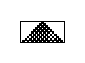
\includegraphics[width=3.0in,height=1.5in]{figs/rule50.eps}}
\afterfig

The first row shows the state of the system during the first
timestep; it starts with one cell ``on'' and the rest ``off''.
The second row shows the state of the system during the
next time step, and so on.

The triangular shape in the figure is typical of these CAs; is it a
consequence of the shape of the neighborhood.  In one time step, each
cell influences the state of one neighbor in either direction.  During
the next time step, that influence can propagate one more cell in each
direction.  So each cell in the past has a ``triangle of influence''
that includes all of the cells that can be affected by it.


\section{Implementing CAs}

To generate the previous figure, I wrote a Python program that
uses the NumPy and PyLab packages.  NumPy provides a
data structure called an {\bf array}; PyLab provides the plotting
functions I used to generate the figure.  
You can download my code from \url{thinkcomplex.com/CA.py}.

An array is a multi-dimensional data structure whose elements
are all the same type.  It is simular to a nested list, but it
is usually smaller and faster.  The following figure shows why:

[Will someone please send me a nice figure in .fig or a similar
format?]

\vspace{3in}

The diagram on the left shows a list of lists of integers; the
diagram on the right shows an array of the same integers.  Because
all of the elements are the same type, they are all the same size,
so they are stored contiguously in memory.  This arrangement
saves space because it stores the elements directly rather
than by reference.  It saves time because the location
of an element can be computed directly from the indices; there
is no need to follow a series of references.

Here is a definition of a CA that uses an array to store the states
of the cells:

\begin{verbatim}
from numpy import *
import pylab

class CA(object):

    def __init__(self, n=100):
        self.n = n
        self.m = n*2 + 1
        self.array = zeros((n, self.m), dtype=int8)
        self.array[0, self.m/2] = 1
        self.next = 1
        self.table = make_table()
\end{verbatim}

{\tt n} is the number of rows in the array, which is the number
of timesteps we will compute.  {\tt m} is the number of columns,
which is the number of cells.  At least to get started, we will implement
a finite sequence of cells.

{\tt zeros} is provided by NumPy; it creates a new array with
the given dimensions, {\tt n} by {\tt m}.  Arrays can have any
number of dimensions, but let's start small.  {\tt dtype} stands
for ``data type,'' and is specifies the type of the array elements.
{\tt int8} is an 8-bit integer, so we are limited to 256 states,
but that's no problem: we only need two.

Array indexing is similar to list indexing.  The line

\begin{verbatim}
        self.array[0, self.m/2] = 1
\end{verbatim}
%
turns the cell in the middle of the first row on.  The rest
of the array is all zero.

The attribute {\tt next} keeps track of the next row of the
array---the one that will be filled in during the next timestep.

\verb"make_table" builds a dictionary that maps from the state
of the neighborhood to the next state of the middle cell:

\begin{verbatim}
def make_table():
    d = {}
    d[1,1,1] = 0
    d[1,1,0] = 0
    d[1,0,1] = 1
    d[1,0,0] = 1
    d[0,1,1] = 0
    d[0,1,0] = 0
    d[0,0,1] = 1
    d[0,0,0] = 0
    return d
\end{verbatim}

This example is the table for Rule 50.

CA objects provide a method named 
{\tt step} that computes the next state of the CA:

\begin{verbatim}
    def step(self):
        """execute one time step by computing the next row of the array"""
        i = self.next
        self.next += 1

        for j in xrange(1,self.m-1):
            neighborhood = tuple(self.array[i-1, j-1:j+2])
            self.array[i,j] = self.table[neighborhood]
\end{verbatim}

{\tt i} indicates the row of the matrix, which is the timestep
we are about to compute.  {\tt j} loops through the cells, skipping
the first and last, which are always off.

Arrays support slice operations, so {\tt self.array[i-1, j-1:j+2]}
gets three elements from row {\tt i-1}.
The last line looks up the neighborhood tuple in the table to get
the next state and stores it in the array.

Array indexing is constant time, so {\tt step} is linear in $n$.
Filling in the whole array is $O(nm)$.

You can read more about NumPy and arrays at
\url{scipy.org/Tentative_NumPy_Tutorial}.

CA objects also provide a method named {\tt draw} that uses
PyLab to display a graphical representation of the evolution
of the CA.  The graph is 2-D because it shows the state of the
CA over time (not to be confused with the 2-D CAs we will see
in the next chapter.

\begin{verbatim}
    def draw(self):
        pylab.gray()
        pylab.pcolor(-flipud(self.array))
        pylab.axis([0, self.m, 0, self.n])
        pylab.xticks([])
        pylab.yticks([])
\end{verbatim}

{\tt gray} tells PyLab to use a grayscale color map;
{\tt pcolor} generates a ``pseudocolor'' plot that shows a
rectangle for each element in the array, with a color that
corresponds to the value of the element.  Since the elements
of the array are 0 and 1, the colors are black and white.

{\tt flipup} stands for ``flip up-down;'' it flips the array
so that row 0 is at the time and time flows down, which is the
convention for these plots.  Negating the elements of the array
makes 1 black and 0 white, which is also the convention.

{\tt axis} sets the bounds of the display to fit the dimensions of
the array.  {\tt xticks} and {\tt yticks} specify where the
labels and tick-marks should be on the axes; the empty list means
that we don't want any ticks at all.


\begin{ex}

Download my CA implementation from
\url{thinkcomplex.com/CA.py}
and add a new class called {\tt CircularCA} that extends
{\tt CA} so that the cells are arranged in a ring.

Hint: you might find it useful to add a column of ``ghost cells'' to
the array.

You can download my solution from 
\url{thinkcomplex.com/CircularCA.py}

\end{ex}


\section{Classifying CAs}

Wolfram proposed that the behavior of CAs can be grouped
into four classes.  Class 1 contains the simplest (and least
interesting) CAs, the ones that evolve from almost any starting
condition to the same uniform pattern.  As a trivial example,
Rule 0 always generates an empty pattern after one time step.

Rule 50 is an example of Class 2.  It generates a simple pattern with
nested structure; that is, the pattern contains many smaller versions
of itself.  Rule 18 makes the nested structure even clearer; here is
what it looks like after 64 timesteps:

\beforefig
\centerline{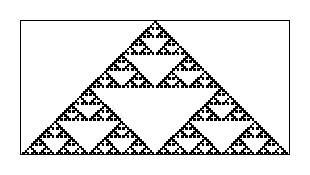
\includegraphics[width=3.0in,height=1.5in]{figs/rule18.eps}}
\afterfig

This pattern resembles the Sierpi\'{n}ski triangle, which 
you can read about at \url{wikipedia.org/wiki/Sierpinski_triangle}.

Some Class 2 CAs generate patterns that are intricate and
aesthetic, but compared to Classes 3 and 4, they are relatively
simple.


\section{Randomness}

Rule 30 is an example of Class 3; here is what it looks like
after 100 timesteps:

\beforefig
\centerline{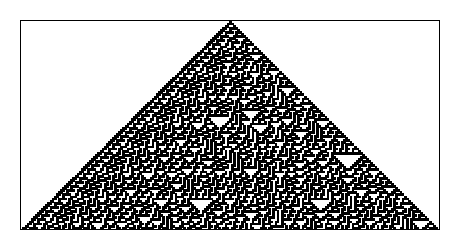
\includegraphics[width=3.0in,height=1.5in]{figs/rule30.eps}}
\afterfig

There is a repeating pattern along the left boundary; in the
center and right there are triangles in various sizes, but if
there is a pattern, it is hard to see.  In fact, if you think it
looks completely random, you may be right.

For example, if you take the center column and treat it as a
sequence of bits, it is hard to distinguish from a truly random
sequence.  It passes many of the statistical tests people use
to test whether a sequence of bits is random.  In fact, the
the computer algebra system Mathematica uses the Rule 30 CA as
a random-number generator.  This choice is not a coincidence:
Wolfram conceived and led the development of Mathematica.

Programs that produce random-seeming numbers are called
{\bf pseudo-random number generators} (PRNGs).  They are not considered
truly random because

\begin{itemize}

\item Many of them produce sequences with regularities that
can be detected statistically.  For example, the original implementation
of {\tt rand} in the C library used a linear congruential generator
that yielded sequences with easily detectable serial correlations.

\item Any deterministic generator that uses a finite amount
of state will eventually repeat itself.  One of the
characteristics of a generator is the {\bf period} of this
repetition.

\item The underlying process is fundamentally deterministic,
unlike some physical processes, like radioactive decay and
thermal noise, that are considered to be fundamentally
random.

\end{itemize}

Modern PRNGs produce sequences that are statistically
indistinguishable from random, and they can be implemented with with
periods so long that the universe will collapse before they repeat.
The existence of these generators raises the question of whether there
is any real difference between a good quality pseudo-random sequence
and a sequence generated by a ``truly'' random process.  In {\em A New
  Kind of Science}, Wolfram argues that there is not (pages 315--326).

\begin{ex}

This exercise asks you to implement and test several PRNGs.

\begin{enumerate}

\item Write a program that implements one of the linear congruential
generators described at
\url{wikipedia.org/wiki/Linear_congruential_generator}).

\item Download {\tt DieHarder}, a random number test suite, from
\url{phy.duke.edu/~rgb/General/rand_rate.php} and use it to
test your PRNG.  How does it do?

\item Read the documentation of Python's {\tt random} module.
What PRNG does it use?  Test it using DieHarder.

\item Implement a Rule 30 CA on a ring with a few hundred cells,
run it for as many time steps as you can in a reasonable amount
of time, and output the center column as a sequence of bits.
Test it using DieHarder.

\end{enumerate}

\end{ex}



\section{Determinism}

The existence of Class 3 CAs is surprising.  To understand how
surprising, it is useful to consider the philosophical stance called
{\tt determinism} (see \url{wikipedia.org/wiki/Determinism}).
Most philosophical stances are hard to define precisely because
they come in a variety of flavors.  I often find it useful
to define them with a list of statements ordered from weak
to strong:

\begin{description}

\item[D1:] Deterministic models can make accurate predictions
for some physical systems.

\item[D2:] Many physical systems can be modeled by deterministic
processes, but some are intrinsically random.

\item[D3:] All events are caused by prior events, but many
physical systems are nevertheless fundamentally unpredictable.

\item[D4:] All events are caused by prior events, and can (at
least in principle) be predicted.

\end{description}

My goal in constructing this range is to make D1 so weak that
virtually everyone would accept it, D4 so strong that almost
no one would accept it, with intermediate statements that
some people accept.

The center of mass of world opinion swings along this
range in response to historical developments and scientific
discoveries.  Prior to the scientific revolution, many people
regarded the working of the universe as fundamentally unpredictable
or controlled by supernatural forces.  After the triumphs of
Newtonian mechanics, some optimists came to believe something
like D4; for example, in 1814 Pierre-Simon Laplace
wrote

\begin{quote}
We may regard the present state of the universe as the effect of its
past and the cause of its future. An intellect which at a certain
moment would know all forces that set nature in motion, and all
positions of all items of which nature is composed, if this intellect
were also vast enough to submit these data to analysis, it would
embrace in a single formula the movements of the greatest bodies of
the universe and those of the tiniest atom; for such an intellect
nothing would be uncertain and the future just like the past would be
present before its eyes.
\end{quote}

This ``intellect'' came to be called ``Laplace's Demon.
\footnote{See \url{wikipedia.org/wiki/Laplace's_demon}.  The word
  ``demon'' in this context has the sense of ``spirit,'' with no
  connotation of malevolence.}''

Discoveries in the 19th and 20th centuries gradually dismantled
this hope.  The thermodynamic concept of entropy, radioactive decay
and quantum mechanics posed successive challenges to strong
forms of determinism.  

In the 1960s chaos theory showed that in some deterministic systems
prediction is only possible over short time scales,  limited by
the precision of measurements of initial conditions.

Most of these systems were continuous in space (if not time)
and nonlinear, so the complexity of their behavior was not
entirely suprising.  Wolfram's demonstration of
complex behavior in simple cellular automata is
more surprising---and disturbing, at least to a classical
world view.

So far I have focused on scientific challenges to determinism, but the
longest-standing objection is the conflict between
determinism and human free will.  Complexity science provides
an approach that may resolve this apparent conflict, but I
will stop there for now.


\section{Structures}

If you agree that Class 3 CAs are surprising, then Class 4 will blow
your mind.  It turns out that several 1-D CAs, most notably Rule 110,
are {\bf Turing complete}, which means that they can compute any
computable function.  This property, also called {\bf universality},
was proved by Matthew Cook in 1998.

Here is a what Rule 110 looks like with an initial condition of
a single cell and 100 timesteps:

\beforefig
\centerline{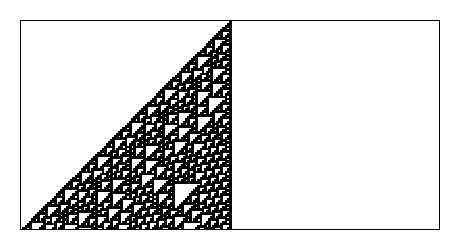
\includegraphics[width=3.0in,height=1.5in]{figs/rule110.eps}}
\afterfig

At this time scale it is not apparent that anything special is
going on.  There are some regular patterns but also some features
that are hard to characterize.

Here is a bigger picture, starting with a random initial
condition and 600 timesteps:

\beforefig
\centerline{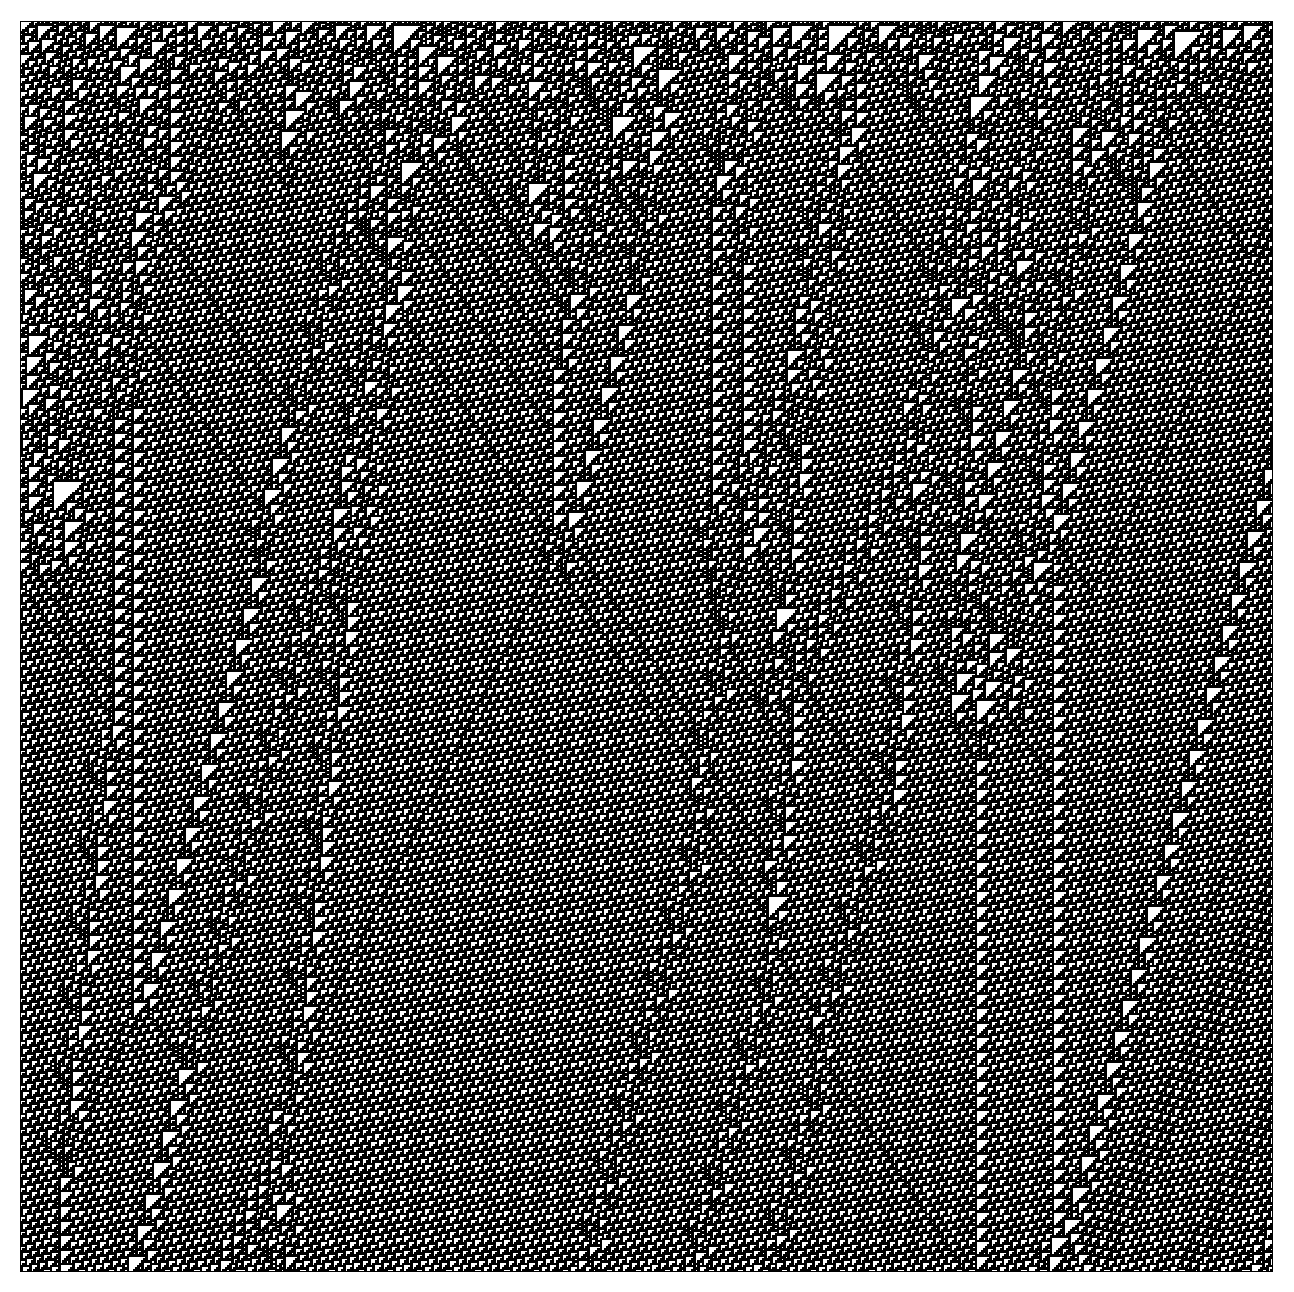
\includegraphics[width=5.5in,height=5.5in]{figs/rule110random.eps}}
\afterfig

After about 100 steps the background settles into a simple repeating
pattern, but there are a number of persistent structures that appear
as disturbances in the background.  Some of these structures
are stable, so they appear as vertical lines.  Others translate in
space, appearing as diagonals with different slopes, depending on
how many time steps they take to shift by one column.  These
structures are sometimes called {\bf spaceships}.

Collisions between spaceships yield different results
depending on the types of the spaceships and the phase they are in
when the collide.  Some collisions annihilate both ships; others
leave one ship unchanged; still others yield one or more ships of
different types.

These collisions are the basis of computation in a Rule 110 CA.  If
you think of spaceships as signals that propagate on wires, and
collisions as gates that compute logical operations like AND and OR,
you can get a sense of what it means to perform a computation.
To get a sense of how Cook proved the universality of Rule 110,
see \url{wikipedia.org/wiki/Rule_110_cellular_automaton}


\begin{ex}

This exercise asks you to experiment with Rule 110 and see how
many spaceships you can find.

\begin{enumerate}

\item Modify your program from the previous exercises so it
starts with the initial condition that yields the stable
background pattern.

\item Modify the initial condition by adding different patterns in the
  center of the row and see which ones yield spaceships.  You might
  want to enumerate all possible patterns of $n$ bits, for some
  reasonable value of $n$.  For each spaceship, can you find the
  period and rate of translation?  What is the biggest spaceship you
  can find?

\end{enumerate}

\end{ex}


\section{Universality}

To understand universality, we have to understand
computability theory, which is about models of
computation and what they compute.

One of the most general models of computation is the Turing machine,
which is an abstract computer proposed by 
Alan Turing in 1936.  A Turing machine is a 1-D CA, infinite in both
directions, augmented with a read-write head.  At any time, the head
is positioned over a single cell.  It can read the state of that cell
(usually there are only two states) and it can write a new value into
the cell.

In addition, the machine has a register, which records which
of a finite number of states the machine is in, and a table
of rules.  For each machine state and cell state, the table
specifies an action.  Actions can include modifying the cell
the head is over and moving one cell to the left or right.

A Turing machine is not a practical design for a computer, but it
can be used as a model of common computer architectures.  For
a given program running on a real computer, it is possible
(at least in principle) to construct a Turing machine that performs
an equivalent computation.

The Turing machine is useful because it is possible to characterize
the set of functions that can be computed by a Turing machine,
which is what Turing did.  Functions in this set are
called Turing computable.

To say that a Turing machine can compute any Turing-computable
function is a {\bf tautology}: it true by definition.  But
Turing-computability is more interesting than that.

It turns out that just about every reasonable model of computation
anyone has come up with is Turing complete; that is, it can compute
exactly the same set of functions as the Turing machine.
Some of these models, like lamdba calculus, are very different
from a Turing machine, so their equivalence is surprising.

This observation led to the Church-Turing Thesis, which is
essentially a definition of what it means to be computable.
The ``thesis'' is that Turing-computability is the right,
or at least natural, definition of computability, because 
it describes the power of such a diverse collection of models
of computation.

The Rule 110 CA is yet another model of computation, and remarkable
for its simplcity.  That it, too, turns out to be universal lends
support to the Chuch-Turing Thesis.

In {\em A New Kind of Science}, Wolfram states a variation of this
thesis, which he calls the ``principle of computational equivalence:''

\begin{quote}
Almost all processes that are not obviously simple can be viewed as
computations of equivalent sophistication.

More specifically, the principle of computational equivalence says
that systems found in the natural world can perform computations up to
a maximal (``universal'') level of computational power, and that most
systems do in fact attain this maximal level of computational
power. Consequently, most systems are computationally
equivalent\footnote{See
  \url{mathworld.wolfram.com/PrincipleofComputationalEquivalence.html}.}.
\end{quote}

Applying these definitions to CAs, Classes 1 and 2 are ``obviously
simple.''  It may be less obvious that Class 3 is simple, but in a way
perfect randomness is as simple as perfect order; complexity happens
in between.  So Wolfram's claim is that Class 4 behavior is common in
the natural world, and that almost all of the systems that manifest it
are computationally equivalent.


\section{Falsifiability}

Wolfram holds that his principle is a stronger claim than the
Church-Turing Thesis because it is about the natural world rather
than abstract models of computation.  But saying that natural processes
``can be viewed as computations'' strikes me as a statement about
model selection more than a hypothesis about the natural world.

Also, with qualifications like
``almost'' and undefined terms like ``obviously simple,'' his
hypothesis may be {\bf unfalsifiable}.  Falsifiability is
an idea from the philosophy of science, proposed by Karl Popper
as a demarcation between scientific hypotheses and pseudoscience.
A hypothesis is falsifiable if there is an experiment, at least
in the realm of practicality, that would contradict the hypothesis
if it were false.

For example, the claim that all life on earth is descended
from a common ancestor is falsifiable because it makes specific
predictions about similarities in the genetics of modern species
(among other things).  If we discovered a new species whose
DNA was almost entirely different from ours, that would
contradict (or at least bring into question) the theory of
universal common descent.

On the other hand, ``special creation,'' the claim that all species
were created in their current form by a supernatural agent, is
unfalsifiable because there is nothing that we could observe about the
natural world that would contradict it.  Any outcome of any experiment
could be attributed to the will of the creator.  

Unfalsifiable hypotheses can be appealing, at first, because
they are impossible to refute.  If your goal is never to be
proved wrong, you should choose hypotheses that are as
unfalsifiable as possible.

But if your goal is to make reliable predictions about the world---and
this is at least one of the goals of science---then unfalsifiable
hypotheses are useless.  The problem is that they have
no consequences (if they had consequences, they would be
falsifiable).

For example, if the theory of special creation were true, what good
would it do me to know it?  It wouldn't tell me anything about the
creator except that he has an ``inordinate fondness for beetles.
\footnote{Attributed to J. B. S. Haldane.}''  And unlike the
theory of common descent, which informs many areas of science
and engineering, it would be of no use for understanding
the world or acting in it.

\begin{ex}

Falsifiability is an appealing and useful idea, but among
philosophers of science it is not generally accepted 
as a solution to the demarcation problem, as Popper claimed.

Read \url{wikipedia.org/wiki/Falsifiability} and answer the following questions.

\begin{enumerate}

\item What is the demarcation problem?

\item How, according to Popper, does falsifiability solve the
demarcation problem?

\item Give an example of two theories, one considered scientific
and one considered unscientific, that are successfully distinguished
by the criterion of falsifiability.

\item Can you summarize one or more of the objections that 
philosophers and historians of science have raised to Popper's
claim?

\item Do you get the sense that practicing philosophers think
highly of Popper's work?

\end{enumerate}

\end{ex}



\section{What is this a model of?}

Some cellular automata are primarily mathematical artifacts.
They are interesting because they are surprising, 
or useful, or pretty, or because they provide tools for
creating new mathematics (like the Church-Turing thesis).

But it is not clear that they are models of physical systems.  And if
they are, they are highly abstracted, which is to say that they are
not very detailed or realistic.  For example, some species of cone
snail\footnote{See \url{en.wikipedia.org/wiki/Cone_snail}} produce a
pattern on their shells that resembles the patterns generated by
cellular automata.  So it is natural to imagine that a CA is a model
of the mechanism that produces patterns on shells as they grow.  But,
at least initially, it is not clear how the elements of the model
(cells, communication between neighbors, rules) correspond to the
elements of a growing snail.

For conventional physical models, being realistic is a virtue, at
least up to a point.  If the elements of a model correspond to the
elements of a physical system, there is an obvious analogy between the
model and the system.  In general, we expect a model that is more
realistic to make better predictions and to provide more believable
explanations.

Of course, this is only true up to a point.  Models that are
more detailed are harder to work with, and less likely to be
amenable to analysis.  At some point, a model can be so complex
that it is easier to experiment with a real system.

At the other extreme, simple models can be compelling
exactly because they are simple.  

Simple models offer a different kind of explanation than detailed
models.  With a detailed model, the argument goes something
like this: ``We are interested in physical system S, so we
construct a detailed model, M, and show by analysis and simulation
that M exhibits a behavior, B, that is similar (qualitatively
and/or quantitatively) to an observation of the real system, O.
So why does O happen?  Because S is similar to M, and
B is similar to O, and we can prove that M leads to B.''

With simple models we can't claim that S is similar to M, because it
isn't.  Instead, the argument goes like this: ``There is a set of
models, ${M_0, M_1, ...}$ that share a common set of features, ${F_0,
  F_1, ...}$.  
Any model that has these features will exhibit some
behavior, B.  $M_0$ is the simplest model that has all of these
features and exhibits B.  If we make an observation, O, that
resembles B, one way to explain it is to show that the system,
S, has the minimum set of features, in common with $M_0$, that
produce B.''

For this kind of argument, 
adding more features doesn't help.  Making the model more
realistic doesn't make the model more reliable; it only
obscures the difference between the essential features that
cause O and the incidental features that are particular to
S.

\chapter{Games of Life}


\section{Abstract classes}

In the previous chapter we used PyLab to generate a graphical
representation of the evolution of a 1-D cellular automaton.  Using
{\tt pylab.pcolor} is easy but for large numbers of cells the
performance is a little slow.  Also, the Postscript PyLab generates is
not very efficient.  For the figures in this book, I wrote some Python
code that generates small, fast Postscript.
Along the way, I also wrote code to generate GIF images using
the Python Imaging Library (PIL).

I ended up with three different ways to draw a CA, and it was
a challenge to organize the code in a sensible way.  I ended up
using a design pattern called an {\bf abstract type} (see
\url{wikipedia.org/wiki/Abstract_type}).

An abstract type is a class definition that defines an interface, but
leaves the implementation of the interface unspecified.  As an
example, here is the definition of a class named {\tt Drawer}:

\begin{verbatim}
class Drawer(object):

    def draw(self, ca):
        """draw a representation of cellular automaton (ca).
        This function generally has no visible effect."""
    
    def show(self):
        """display the representation on the screen, if possible"""

    def save(self, filename):
        """save the representation of the CA in (filename)"""        
\end{verbatim}

These methods have no statements in the body, only dosctrings.
It is up to the subclasses to provide implementations.
In my program, I defined three subclasses that inherit from
Drawer: PyLabDrawer, which uses {\tt pylab.pcolor}, 
PILDrawer, which uses PIL and Tkinter to generate and display
a GIF, and EPSDrawer, which generates encapsulated postscript.

Some programming languages provide explict support for abstract types,
so they can generate appropriate error messages if something goes
wrong.  For example, it is usually illegal to instantiate an abstract
type---it doesn't provide an implementation, so it can't really do
anything.  Python does not enforce this rule, so it is possible (but
not very useful) to instantiate a Drawer.  In Python, it is up to the
programmer to use abstract types correctly.


\begin{ex}
Can you think of a way to change the definition of Drawer
so that it raises an exception if you try to instantiate it?
\end{ex}


\begin{ex}

Rewrite your code from the previous chapter using {\tt Drawer}
as an abstract type.  One of the advantages of this reorganization
is that you can separate the CA code from the
graphics code.  All of the code that pertains to PyLab should
be moved into the definition of {\tt PyLabDrawer}.

Then write another implementation of a {\tt Drawer} that uses PIL
to generate a GIF.  To get you started, you can download
\url{thinkcomplex.com/pil.py}, which contains example
code that creates an image, draws a rectangle, displays the
image using Tkinter, and generates a GIF.

Finally, if you are familiar with Postscript, write a third
implementation of {\tt Drawer} that generates encapsulated
Postscript.  Or you might consider writing an implementation using
a Tkinter Canvas.

You can download my solution from
\url{thinkcomplex.com/CADrawer.py}

\end{ex}



\section{Conway}

One of the first cellular automata to be studied, and probably the
most popular of all time, 2-D CA called ``The Game of Life,'' or GoL
for short.  It was developed by John H. Conway and popularized in 1970
in Martin Gardner's column in {\em Scientific American}.

The cells in GoL are arranged in a 2-D grid, either infinite in both
directions or wrapped in both directions.  A grid that is wrapped
in both directions is called a {\bf torus} because it is topographically
equivalent to the surface of a doughnut (see \url{wikipedia.org/wiki/Torus}).

Each cell has two states---live and dead---and 8 neighbors---north,
south, east, west, and the four diagonals.  This set of neighbors
is sometimes called a Moore neighborhood.

The rules of GoL are {\bf totalistic}, which means that the next
state of a cell depends on the number of live neighbors only, 
not on their arrangement.  The following table summarizes the
rules:

\begin{tabular}{|l|c|c|}
\hline
Number of     &   Current      & Next \\
neighbors     &   state        & state \\
\hline
2--3          &   live           & live         \\
0--1,4--8     &   live           & dead         \\
3             &   dead           & live         \\
0--2,4--8     &   dead           & dead         \\
\hline
\end{tabular}

GoL turned out to be popular because

\begin{itemize}

\item There are a number of simple initial conditions that yield
surprisingly complex behavior.

\item There are a number of interesting stable patterns: some
oscillate (with various periods) and some translate like the
spaceships in Wolfram's Rule 110 CA.

\item Like Rule 110, GoL is Turing complete.

\item Conway posed an intriguing conjecture---that there is
no initial condition that yields unbounded growth in the number
of live cells---and offered \$50 to anyone who could prove
or disprove it.

\item The increasing availability of computers made it possible
to automate the computation and display the results graphically.
That turns out to be more fun that Conway's original implementation
using a checkerboard.

\end{itemize}


\begin{ex}

Write a class that implements a ``Game of Life'' CA, and another
class that displays an animated sequence of timesteps on the screen.

Remember that all cells have to be updated ``simultaneously;'' for
example, if you traverse an array and update cells as you go, you
will end up using some new values in subsequent updates.  The
result is not a correct implementation of Conway's rules.

There are many implementation options:

\begin{itemize}

\item For the data structure that stores the state of the CA, you
could use a NumPy array, a list of lists, a dictionary, or even
a PIL Image.  If you choose a PIL Image, you might find
{\tt ImageFilter.Kernel} useful.

\item To display the CA, you could use PyLab, PIL, Postscript, or
{\tt CellWorld}, which is part of Swampy.

\end{itemize}

Try to choose an implementation that can update and display a large CA
quickly\footnote{For some speed tips, see Alan Hensel's implementation
or check out HashLife.}.

Start the CA in a random state and run it until it stabilizes.
What stable patterns can you identify?

\end{ex}


\section{Life patterns}

If you run GoL from a random starting state, a number of stable
patterns are likely to appear.  Blocks, boats, beehives, blinkers and
gliders are among the most common.  People have spent embarassing
amount of time finding (and naming) these patterns.  If you search
the web, you will find many collections.

\begin{ex}

Many named patterns are available in portable file formats.
Modify your program to parse one of them in order to place patterns
into your grid and run them.

\end{ex}

From most initial conditions, GoL quickly reaches a stable
state where the number of live cells is nearly constant
(usually with a small amount of oscillation).

But there are a some simple starting conditions that take a
long time to settle down and yield a surprising
number of live cells.  These patterns are called ``Methuselahs''
because they are so long-lived.  One of the simplest is the
r-pentomino, which has only five cells in the shape of a ``r,'' hence
the name.  It runs for 1103 steps and yields 6 gliders, 8 blocks, 4
blinkers, 4 beehives, 1 boat, 1 ship, and 1 loaf.
One of the longest-lived small patterns is rabbits, which starts
with 9 live cells and takes 17 331 steps to stabilize.


\section{Conway's conjecture}

These long-lived patterns bring us back to Conway's original question:
are there initial patterns that never stabilize?  Conway thought not,
but he described two kinds of pattern that would prove him wrong, a
``gun'' and a ``puffer train.''  A gun is an stable pattern that
periodically produces a spaceship---as the stream of spaceships moves
out from the source, the number of live cells grows indefinitely.  A
puffer train is a translating pattern that leaves live cells in its
wake.

It turns out that both of these patterns exist.  A team led
by Bill Gosper discovered the first, a glider gun now called
Gosper's Gun.  Gosper also discovered the first puffer train.
You can find descriptions and animations of these patterns
in several places on the Web.

There are many patterns of both types, but they are not easy to
design or find.  That is not a coincidence.  Conway chose the
rules of GoL so that his conjecture would not be obviously
true or false.  Of all the possible rules for a 2-D CA, most
yield simple behavior; most initial conditions stabilize quickly
or grow unboundedly.  By avoiding uninteresting CAs, Conway
was also avoiding Wolfram's Class 1 and Class 2 behavior, and
probably Class 3 as well.

If we believe Wolfram's Principle of Computational Equivalence, we
should expect GoL to be in Class 4.  And it is.  The Game of Life was
proven to be Turing complete in 1982 (and again, independently in
1983).  Since then several people have constructed GoL patterns that
implement a Turing machine or another machine known to be Turing
complete.



\section{Realism}

Stable patterns in GoL are hard not to notice, especially the ones
that move.  It is natural to think of them as persistent entities, but
remember that a CA is made of cells; there is no such thing as a toad
or a loaf.  Gliders and other spaceships are even less real because
they are not even made up of the same cells over time.  So these
patterns are like constellations of stars.  We perceive them because
we are good at seeing patterns, or because we have active
imaginations, but they are not real.

Right?

Well, not so fast.  Many entities that we consider
``real'' are also persistent patterns of entities at a smaller
scale.  Hurricanes are just patterns of air flow, but we give
them personal names!  And people, like gliders, are not made
up of the same cells over time.  But even if you replace every
cell in your body, we consider you the same person.

This is not a new observation---about 2500 years ago Heraclitus
pointed out that you can't step in the same river twice---but the
entities that appear in the Game of Life are a useful test case for
thinking about {\bf philosophical realism}.

In the context of philosophy, realism is the view that entities
in the world exist independent of human perception and conception.
By ``perception'' I mean the information that we get from
our senses, and by ``conception'' I mean the mental model
we form of the world.  For example, our vision systems perceive
something like a 2-D projection of a scene, and our brains
use that image to construct a 3-D model of the objects in the
scene.

{\bf Scientific realism} pertains to scientific theories and the
entities they posulate.  Again, I find it useful to state
philosophical positions in a range of strengths, where SR1 is
a weak form of scientific realism and SR4 is a strong form:

\begin{description}

\item[SR1:] Scientific theories are true or false to the degree that
  they approximate reality, but no theory is exactly true.  Some
  postulated entities may be real, but there is no principled way to
  say which ones.

\item[SR2:] As science advances, our theories become better
  approximations of reality.  At least some postulated entities are
  known to be real.

\item[SR3:] Some theories are exactly true; others are approximately
  true.  Entities postulated by true theories, and some entities
  in approximate theories, are real.

\item[SR4:] A theory is true if it describes reality correctly, and
  false otherwise.  The entities postulated by true theories are real;
  others are not.

\end{description}

SR4 is so strong that it is probably untenable; by such a strict
criterion, almost all current theories are known to be false.  
Most realists would accept something in the space
between SR1 and SR3.


\section{Instrumentalism}

But SR1 is so weak that it verges on {\bf instrumentalism}, which is
the view that we can't say whether a theory is true or false because
we can't know whether a theory corresponds to reality.  Theories are
instruments that we use for our purposes; a theory is useful, or not,
to the degree that it is fit for its purpose.

To see whether you are comfortable with instrumentalism, consider
the following statements:

\begin{quote}
``Entities in the Game of Life aren't real; they are just patterns of
  cells that people have given cute names.''
\end{quote}

\begin{quote}
``A hurricane is just a pattern of air flow, but it is a useful
  description because it allows us to make predictions and communicate
  about the weather.
\end{quote}

\begin{quote}
``Freudian entities like the Id and the Superego aren't real, but they
  are useful tools for thinking and communicating about psychology (or
  at least some people think so).''
\end{quote}

\begin{quote}
``Electrons are postulated entities in our best theories of
electro-magnetism, but they aren't real.  We could construct
other theories, without postulating electrons, that would be
just as useful.''
\end{quote}

\begin{quote}
``Many of the things in the world that we identify as objects are
  abritrary collections like constellations.  For example, a mushroom
  is just the fruiting body of a fungus, most of which grows
  underground as a barely-contiguous network of cells.  We focus
  on mushrooms for practical reasons like visibility and edibility.''
\end{quote}

\begin{quote}
``Some objects have sharp boundaries, but many are fuzzy.  For
  example, which molecules are part of your body: Air in your lungs?
  Food in your stomach?  Nutrients in your blood?  Nutrients in a
  cell?  Water in a cell?  Structural parts of a cell?  Hair?  Dead
  skin?  Dirt?  Bacteria on your skin?  Bacteria in your gut?
  Mitochondria?  How many of those molecules do you include when you
  weigh yourself.  Conceiving the world in terms of discrete objects
  is useful, but the entities we identify are not real.''
\end{quote}

Give yourself one point for each statement you agree with.
If you score 4 or more, you might be an instrumentalist!

If you are more comfortable with some of these statements than with
others, ask youself why.  What are the differences in these
scenarios that influence your reaction?  Can you make
a principled distinction between them?

\begin{ex}

Read the Wikipedia page on instrumentalism and construct a sequence
of statements that characterize instrumentalism in a range of
strengths.

\end{ex}


\section{Turmites}

If you generalize the Turing machine to two dimensions or
add a read-write head to a 2-D CA, either way you get a
cellular automaton called a Turmite.  It is named after a
``termite'' because of the way the read-write head moves, but
spelled wrong as an homage to Turing. 

One of the most famous Turmites is Langton's Ant, discovered
by Chris Langton in 1986.  The ant is a read-write head with
four states, which you can think of as facing north, south,
east or west.  The cells have two states, black and white.

The rules are simple.  During each time step, the ant checks the color
of the cell is it on.  If it is black, the ant turns to the right,
changes the cell to white, and moves forward one space.  If the cell
is white, the ant turns left, changes the cell to black, and moves
forward.

Given a simple world, a simple set of rules, and only one moving part,
you might expect to see simple behavior---but you should know
better by now.  Starting with all white cells, Langton's ant
moves in a seemingly random pattern for more than 10 000 steps
before it enters a cycle with a period of 104 steps.  After
each cycle, the ant is translated diagonally, so it leaves
a linear trail called the ``highway.''

If you start with multiple Turmites, they interact with each
other in seemingly complex ways.  If one Turmite is on the
highway, another can follow it, overtake it, and cause it to
reverse its pattern, moving back up the highway and leaving
only white cells behind.  

\begin{ex}

Read \url{wikipedia.org/wiki/Langton's_ant}.

Swampy includes a module called {\tt TurmiteWorld} that contains
an implementation of Langton's Ant.  Read the code to get a sense
of how it works, then run it with a variety of initial conditions.

\end{ex}


\section{Percolation}

The CAs we have seen so far are not physical models; that is, they are
not intended to describe systems in the real world.  As it turns out,
there are some real systems that have the same structure as a CA.  For
example, Wolfram has argued that patterns on some animals, especially
cone snails, may be generated by processes that are equivalent to a CA
(see
\url{stephenwolfram.com/publications/articles/ca/83-cellular/2/text.html}).

But some CAs are designed explicitly as physical models.  In this
section we will consider a simple grid-based model of percolation;
in the next chapter we will see examples that model forest fires,
avalanches, and earthquakes.

Percolation is a process in which a fluid flows through a semi-porous
material.  Examples include oil in porous rock, water in paper, and
hydrogen gas in micropores.  Percolation models are also used to study
systems that are not literally percolation, including epidemics and
networks of electrical resistors.

Percolation processes often exhibit a phase change; that is, an
abrupt transition from one behavior (low flow) to another
(high flow) with a small change in a continuous parameter (like
the porosity of the material).  This transition is sometimes
called a ``tipping point.''

There are two common models of these systems: bond percolation
and site percolation.  Bond percolation is based on a square lattice
of sites, where each site is connected to four neighbors by
a bond.  Each bond is either porous or non-porous.  A set of sites
that are connected (directly or indirectly) by porous bonds is
called a cluster.  In the vocabulary of graphs, a site is a vertex,
a bond is an edge, and a cluster is a connected subgraph.

Site percolation is based on a grid of cells, where each cell
represents a porous
segment of the material or a non-porous segment.  If two porous
cells are adjacent, they are considered connected; a set of
connected cells is considered a cluster.

The rate of flow in a percolation system is primarily determined by
whether or not the porous cells form a path all the way through the
material, so it is useful to know whether a set of cells (or bonds)
contains a ``spanning cluster.''  There are several possible
definitions of a spanning cluster; the choice depends on the system
you are trying to model. The simplest choice is a cluster that reaches
the top and bottom row of the grid.

To model the porosity of the material, it is common to define
a parameter, $p$, which the possibility that any cell (or bond)
is porous.  For a given value of $p$, you can estimate 
$R(p)$, which is the probability that there is a spanning cluster,
by generating a large number of random grids and computing the
fraction that contain a spanning cluster.  This way of estimating
probabilities is called a ``Monte Carlo simulation'' because
it a similar to a game of chance.

Percolation models are often used to compute the critical value,
$p_c$, which is the fraction of porous segments where the phase
change occurs; that is, where the probability of a spanning cluster
increases quickly from near 0 to near 1.

\begin{ex}

The paper ``Efficient Monte Carlo Algorithm and High-Precision Results
for Percolation,'' by Newman and Ziff, presents an efficient algorithm
for checking whether there is a path through a grid.  Read this
paper, implement their algorithm, and see if you can reproduce their
Figure 2(a).

\begin{enumerate}

\item What is the difference between what Newman and Ziff call the
  ``microcanonical ensemble'' and the ``canonical
  ensemble''\footnote{You might find it useful to read about the use of
    these terms in statistical mechanics:
    \url{wikipedia.org/wiki/Statistical_mechanics}.}?  Which one is
  easier to estimate by Monte Carlo simulation?

\item What algorithm do they use to merge two clusters efficiently? 

\item What is the primary reason their algorithm is faster than the
  simpler alternative?

\end{enumerate}
 
\end{ex}



\chapter{Self-organized criticality}

\section{Bak, Tang and Wiesenfeld}

In 1987 Bak, Tang and Wiesenfeld published a paper in Physical Review
Letters, ``Self-organized criticality: an explanation of $1/f$ noise.''
The title takes some explaining.  A system is ``critical'' if it is
in transition between two phases; for example, water at exactly
its freezing point is a critical system.

A wide variety of critical systems demonstrate a few common
behaviors:

\begin{itemize}

\item Long-tailed distributions of some physical quantities: for
  example, in freezing water the distribution of crystal sizes is
  characterized by a power law.

\item Fractal geometries: freezing water tends to form fractal
  patterns---the canonical example is a snowflake.  Fractals
  are characterized by self-similarity; that is, parts of the
  pattern resemble scaled copies of the whole.

\item Variations in time that exhibit pink noise: what we call
  ``noise'' is a time series with many frequency components.  In
  ``white'' noise, all of the components have equal power.  In
  ``pink'' noise, low-frequency components have more power than
  high-frequency components.  Specifically, the power at frequency $f$
  is proportional to $1/f$.  Visible light with this power spectrum
  appears pink, hence the name.

\end{itemize}

Critical systems are usually unstable.  For example, to keep
water in a partially frozen state requires active control of
the temperature.  If the system is left near the critical
temperature, any small deviation will tend to move the system
into one phase or the other.

Many natural systems exhibit behaviors indicative of
criticality, but if critical points are unstable, they should
not be common in nature.  This is the puzzle Bak, Tang and
Wiesenfeld addressed.  Their solution is called self-organized
criticality (SOC), where ``self-organized'' means that from
any initial condition, the system tends to move toward a
critical state and stay there, without external control.

As an example, they propose a model of a sand pile.  The model
is not a very realistic description of a real sand pile, but
it has become the standard example of self-organized criticality.

The model is a 2-D cellular automaton where the state of each cell,
$z(i,j)$, represents the slope of a part of a sand pile.  During each
time step, each cell is checked to see whether it exceeds some
critical value, $K$.  If so, an ``avalanche'' occurs that transfers
sand to neighboring cells; specifically, $z(i,j)$ is decreased by 4,
and each of the 4 neighbors is increased by 1.

At the perimeter of the grid, all cells are kept at $z=0$, so
the excess spills over the edge.  To initialize the system,
Bak et al. start with all $z > K$ and evolve the system until
it stabilizes.  Then they observe the effect of small perturbations;
they choose a cell at random, increment its value
by 1, and evolve the system, again, until it stabilizes.

For each perturbation, they measure $D$, the total number
of cells that are affected by the resulting avalanche.  Most of
the time, $D$ is very small, usually 1.  But occasionally
there is a large avalanche that affects a substantial fraction
of the grid.  The distribution of $D$ turns out to be long-tailed,
which supports the claim that the system is in a critical state.

\begin{ex}

Read the paper and write a program that implements their CA.
See if you can reproduce their Figure 2(a).

What happens if you start all cells in state $z=0$?

\end{ex}


\section{Spectral density}

To understand $1/f$ noise, we have to take a detour to understand
spectral density.  If $h(t)$ is a signal that varies in time, it can
be described by its power spectral density, $P(f)$, which is a
function that maps from a frequency, $f$, to the amount of power the
signal contains at that frequency.

This analysis applies to any varying signal, but I will use sound as
an example.  The note we call ``middle A'' corresponds to a frequency
of 440 cycles per second, or Hertz (Hz).  If you strike a middle A
tuning fork, it produces a sound that is close to a pure sine wave at
440 Hz.  But if you play the same note on a piano, what you hear is
actually a complex sound that contains components at many different
frequencies.  The frequency with the most power is 440, which is why
we perceive the sound as a middle A, but there are also components at
660, 880, and many higher frequencies.  These components are called
``harmonics.''

What we identify as the pitch of a sound is usually the dominant
frequency component.  But if a sound contains many different
components with roughly the same power, it has no particular pitch.
To our ears, it sounds like noise.

Spectral analysis is the process of taking a signal and computing its
spectral density\footnote{The presentation here follows Press et al,
  {\em Numerical Recipes in C}.}.  The first step is to compute the
  Fourier transform of $h(t)$:

\[ H(\omega) = \int_{-\infty}^{\infty} h(t) e^{i \omega t} dt \]

where $\omega = 2 \pi f$ is the angular frequency in
radians per second (rather than cycles per second).  The advantage
of working with angular frequency is that it reduces the number
of times the term $2 \pi$ appears.

$H(\omega)$ is written with a capital letter because it is a complex
number, which you can think of as a vector with a magnitude,
$|H(\omega)|$, and an angle.  The power spectral density is related to
the Fourier transform by the following relation:

\[ P(f) = |H(2 \pi f)|^2 \]

Depending on the application, we may not care about the difference
between $f$ and $-f$.  In that case, we would use the one-sided
power spectral density:

\[ P(f) = |H(2 \pi f)|^2 + |H(-2 \pi f)|^2 \]

So far we have assumed that $h(t)$ is a continuous function, but
often it is a series of values at discrete times.  In that
case we can replace the continuous Fourier transform with
the discrete Fourier transform (DFT).  Suppose that we have
$N$ values $h_k$ with $k$ in the range from 0 to $N-1$.  The
DFT is written $H_n$, where $n$ is an index related to frequency:

\begin{equation}
\label{dft}
H_n = \sum_{k=0}^{N-1} h_k e^{2 \pi i k n / N}
\end{equation}


Each element of this sequence corresponds to a particular frequency.
If the elements of $h_k$ are equally spaced in time, with time
step $d$, the frequency that corresponds to $H_n$ is

\[ f_n = \frac{n}{N d} \]

To get the one-sided power spectral density, you can compute $H_n$
with $n$ in the range $-N/2$ to $N/2$, and

\[ P_n = |H_n|^2 + |H_{-n}|^2 \]

To avoid negative indices, it is conventional to compute
$H_n$ with $n$ in the range $0$ to $N-1$ and use the relation
$H_{-n} = H_{N-n}$ to convert.

\begin{ex}

Write a function named {\tt dft} that takes $h$, a sequence of $N$
values, and returns the sequence $H_n$ with $n$ in the range $0$ to
$N-1$.

Python provides support for complex numbers as a built-in type.
The function {\tt complex} takes two arguments, a real part
and an imaginary part, and returns a complex number:

\begin{verbatim}
>>> complex(1, 1)
(1+1j)
\end{verbatim}

The {\tt cmath} module provides math functions that support
complex numbers:

\begin{verbatim}
>>> import cmath
>>> i = complex(0, 1)
>>> N = 128
>>> cmath.exp(2 * math.pi * i / N)
(0.99879545620517241+0.049067674327418015j)

\end{verbatim}

What is the order of growth run time of {\tt dft}?

\end{ex}


\section{Fast Fourier Transform}
 
The Fast Fourier Transform (FFT) is an efficient algorithm for
computing the DFT.  It is often attributed to Cooley and Tukey,
but it was independently discovered several times earlier.

The first step toward the FFT is to rewrite Equation~\ref{dft}
with the substitution $W = e^{2 \pi i/N}$:

\begin{equation}
H_n = \sum_{k=0}^{N-1} h_k W^{n k}
\end{equation}

The second step is the Danielson-Lanczos Lemma which states

\[ H_n = H^e_n + W^k H^o_n \]

where $H^e$ is the DFT of the even-indexed elements
of $h$, and $H^o$ is the DFT of the odd-indexed elements.
This lemma follows naturally from the definition of $H_n$; you can see
a proof at \url{mathworld.wolfram.com/Danielson-LanczosLemma.html}.

This lemma suggests a recursive algorithm for evaluating the DFT
of a sequence $h$.  If  $h$ has only a single element, then $H=h$.
Otherwise:

\begin{enumerate}

\item Split $h$ into $h^e$ and $h^o$.

\item Compute $H^e$ and $H^o$ by making two recursive calls.

\item Use the lemma to combine $H^e$ and $H^o$ to form $H$.

\end{enumerate}

If $H$ has $2N$ elements, $H^e$ and $H^o$ have only $N$.
In order to merge them, you have to remember that they are
periodic, so $H^e_{n+N} = H^e_{n}$.  So you can double the
length of a sequence just by concatenating it with itself.

This recursive algorithm is the Fast Fourier Transform.

\begin{ex}

Write a function called {\tt fft} that implements
the Fast Fourier Transform.  To check your function, you
can compare it to the function {\tt fft} provided by
the module {\tt numpy.fft}.

What is the order of growth run time of your implementation?
What is the order of growth for the space required?

\end{ex}

Most FFT implementations use a clever indexing scheme to avoid copying
the sequence; instead, they transform the elements in place.  You can
read \url{wikipedia.org/wiki/Butterfly_diagram} to get the details.

\begin{ex}

Once your {\tt fft} is working, write a function named
{\tt psd} that takes a sequence, $h$, and returns its
one-sided power spectral density, $P$.

\end{ex}


\section{Pink noise}

In a followup paper in 1988, Bak, Tang and Wiesenfeld looked
at a time series $F(t)$, which is the number of cells that
exceed the threshold during each time step.  If I understand
their model, they seed avalanches by incrementing the state
of a random cell at random intervals; for example, there might
be a fixed probability during each time step that a cell
is incremented.  In this model (unlike the previous one) there
may be more than one avalanche at a time.

A plot of $F(t)$ shows that it is noisy, but not completely
random, which is consistent with pink, or $1/f$ noise.
As a stronger test, they plot the power spectral density of
$F$ on a log-log scale.  If $F$ is $1/f$ noise, then

\[ P_n \sim 1 / f_n = \frac{N d}{n} \]

Since the units of time in this model are arbitrary, we
can choose $d=1$.  Taking the log of both sides yields:

\[ \log P_n \sim \log N - \log n \]

So on a log-log scale, the PSD of $1/f$ noise is a straight
line with slope -1.

\begin{ex}

Modify your implementation of the sand pile model to increment
a random cell at random intervals and record the number of cells
that exceed the threshold during each time step.

To estimate the average PSD, you can divide the time series into
chunks of 128 to 256 values, compute the PSD of each chunk, and
average together the PSDs.  Plot the result on a log-log scale
and estimate the slope.

\end{ex}


\section{Forest fire models}

In 1992 Drossel and Schwabl proposed a cellular automaton that is
an abstract model of a forest fire.  Each cell is in one of three
states: empty, occupied by a tree, or on fire.

The rules of the CA are:

\begin{enumerate}

\item An empty cell becomes occupied with probability $p$.

\item A cell with a tree will burn if any of its neighbors
  is on fire.

\item A cell with a tree will spontaneously burn, with
  probability $f$, even if none of its neighbors is on fire.

\item A cell with a burning tree becomes an empty cell in the next
  time step.

\end{enumerate}

\begin{ex}

Implement it and test it.

\end{ex}



\begin{ex}

In a 1989 paper, ``Self-organized criticality in the 'Game of Life',''
Bak, Chen and Creutz present evidence that the Game of Life
is a self-organized critical system.

To replicate their tests, run the GoL CA until it stabilizes,
then choose a random cell and toggle it.  Run the CA until
it stablilizes again, keeping track of $t$, the number
of timesteps it takes, and $s$, the number of cells affected.
Repeat for a large number of trials and plot the distributions
of $t$ and $s$.  Also, see if you can think of an effective
experiment to test for $1/f$ noise.

Some later work has called the conclusions of this paper into
question.  You might want to read Blok, ``Life without bounds,''
at \url{zoology.ubc.ca/~rikblok/lib/blok95b.html}.

\end{ex}


\section{Reductionism and Holism}

The original paper by Bak, Tang and Wiesenfeld is one of
the most frequently-cited papers in the last few decades.
Many new systems have been shown to be self-organized critical,
and the sand-pile model, in particular, has been studied
in detail.

As it turns out, the sand-pile model is not a very good model
of a sand pile.  Sand is dense and not very sticky, so momentum
has a non-negligible effect on the behavior of avalanches.  As
a result, there are fewer very large and very small avalanches
than the model predicts, and the distribution is not long tailed.

Bak has suggested that this observation misses the point.
The sand pile model is not meant to be a realistic model of a sand
pile; it is meant to be a simple example of a broad category of
models.

To understand this point, it is useful to think about two
kinds of models, {\bf reductionist} and {\bf holistic}.  A
reductionist model describes a system by describing its parts
and their interactions.  When a reductionist model is used
as an explanation, it depends on an analogy between the 
components of the model and the components of the system.
For example, to explain why the ideal gas law holds, we can
model the molecules that make up the gas with a large number
of point masses with random velocities.  We can model their
interactions as elastic collisions with no molecular forces.
If you simulate or analyze this model you will find that it
obeys the ideal gas law.

This model is satisfactory as an explanation to the degree that
the molecules in a gas behave like the molecules in the model.
So the argument that this model explains the ideal gas law
is essentially an argument by analogy.

Holisitic models are more focused on similarities between
systems and less focused on the relationship between the system
and its parts.  A holistic approach to modeling often consists
of two steps, not necessarily in this order:

\begin{itemize}

\item Identify a kind of behavior that appears in a variety of
systems. 

\item Find the simplest model that demonstrates that behavior.

\end{itemize}

For example, in {\em The Selfish Gene}, Richard Dawkins suggests that
genetic evolution is just one example of an evolutionary system.  He
identifies the essential elements of the category---discrete
replicators, variability and differential reprodcuction---and proposes
that any system that has these elements will display similar
behavior, including complexity without design.  As another
example of an evolutionary system, he proposes memes, which are
thoughts or behaviors that are ``replicated'' by transmission
from person to person.  As memes compete for the resource of
human attention, they evolve in ways that are similar to
genetic evolution.

Critics of memetics have pointed out that memes are a poor analogy
for genes.  Memes differ from genes in many obvious ways.  But
Dawkins has argued that these differences are beside the point
because memes are not {\em supposed} to be analogous to genes.
Memes and genes are both supposed to be examples of the same
category---evolutionary systems.  The differences between them
emphasize the real point, which is that evolution is a general model
that applies to many seemingly disparate systems.

Bak has made a similar argument that self-organized criticality is a
general model for a broad category of systems.  According to the
Wikipedia, ``SOC is typically observed in slowly-driven
non-equilibrium systems with extended degrees of freedom and a high
level of nonlinearity.''

Many natural systems demonstrate behaviors characteristic of critical
systems.  Bak's explanation for this prevalence is that these systems
are examples of the broad category of self-organized criticality.
There are two ways to support this argument.  One is to build
a realistic model of a particular system and show that the model
exhibits SOC.  The second is to show that SOC is a feature of many
diverse models, and to identify the essential characteristics
those models have in common.

The first approach, which I would characterize as reductionist,
can explain the behavior of a particular system.  The
second, holistic, approach, can explain the prevalence of
criticality in natural systems.  They are different models
with different purposes.

For reductionist models, realism is the primary virtue, and
simplicity is secondary.  For holistic models, it is the other
way around.


\begin{ex}

Read \url{wikipedia.org/wiki/Reductionism}
and \url{wikipedia.org/wiki/Holism}.

\end{ex}


\begin{ex}

In a 1996 paper in Nature, Frette et al report the results of
experiments with rice piles.  They find that some kinds of rice
yield evidence of critical behavior, but others do not.

Similarly, Pruessner and Jensen studied large-scale versions of the
forest fire model (using an algorithm similar to Newman and Ziff's).
In their 2004 paper, ``Efficient algorithm for the forest fire model,''
they present evidence that the system is not critical after all.

How do these results bear on Bak's claim that SOC explains
the prevalence of critical phenomena in nature?

\end{ex}


\begin{ex}

In {\em The Fractal Geometry of Nature}, Benoit Mandelbrot proposes an
alternative explanation for the prevalence of long-tailed
distributions in natural systems.  It may not be, as Bak suggests,
that many systems can generate this behavior in isolation.  Instead
there may be only a few, but there may be interactions between systems
that cause the behavior to propagate.

To support this argument, Mandelbrot points out:

\begin{itemize}

\item Interactions between systems may be characterized by operations
  that are (at least approximately) like convolution.  For example,
  if you choose value $a$ from distribution $A$, and independently
  choose value $b$ from distribution $B$, the distribution of the
  sum is the convolution of $A$ and $B$.

\item Long-tailed distributions are stable under convolution; that is,
  if you convolve a long-tailed distribution with another
  distribution, the result is long-tailed.

\end{itemize}

In a few special cases we can compute the convolution of two
distributions analytically.  For example, the convolution of
two normal distributions is also normal.  But for most pairs
of distributions there is no analytical solution.

Here are some simple simulations you can do to explore the
effect of convolution:

\begin{enumerate}

\item Use the functions in the {\tt random} module to generate values
  from a variety of distributions.  For each pair of distributions,
  $A$ and $B$, choose a value from each, $a$ and $b$, and compute the
  empirical distribution of the sum.  Plot the distribution under
  various transforms to test whether it can be characterized as more
  like a uniform, exponential, Weibull, or Pareto distribution.

\item The Central Limit Theorem says that if you choose a large number
  of values from almost any distribution, the distribution of their
  sum tends toward a normal distribution.  Test this theorem by
  drawing samples from exponential, lognormal and Pareto
  distributions, and see how large the number of values has to be
  before the distribution of the sum looks, at least visually, like a
  normal distribution.

  You might consider using a normal probability plot, which you
  can read about at \url{wikipedia.org/wiki/Normal_probability_plot}.
  
% that Wikipedia page is not very good; I should come back to this
% and provide more info.

\end{enumerate}

Would you characterize Mandelbrot's argument as reductionist
or holist?

\end{ex}


\section{SOC, causation and prediction}

If a stock market index drops by a small fraction of a percent in a
day, there is no need for an explanation.  But if it drops 10\%,
people want to know why.  Plenty of people
on television are willing to offer explanations, but the real
answer may be that there is no explanation.

Day-to-day variability in the stock market shows evidence of
criticality: the distribution of value changes is long-tailed
and the time series exhibits $1/f$ noise.
If the stock market is a self-organized critical system, then we
should expect occasional large changes as part of the ordinary
behavior of the market.

The distribution of earthquake sizes is also long-tailed,
and there are simple models of the dynamics of geological faults
that might explain this behavior.  If these models are right,
they imply that large earthquakes are unexceptional; that is,
they do not require explanation any more than
small earthquakes do.

Similarly, Charles Perrow has suggested that failures in large
engineered systems, like nuclear power plants, are like avalanches
in the sand pile model.  Most failures are small, isolated and
harmless, but occasionally a coincidence of bad fortune yields a
catastrophe.  When big accidents occur, investigators go looking for
the cause, but if Perrow's ``normal accident theory'' is correct,
there may be no cause.

These conclusions are not comforting.  Among other things, they
imply that large earthquakes and some kinds of accidents are
fundamentally unpredictable.  It is impossible to look at the
state of a critical system and say whether a large avalanche
is ``due.''  If the system is in a critical state, then a large
avalanche is always possible.  It just depends on the
next grain of sand.

In a sand-pile model, what is the cause of a large avalanche?
Philosophers sometimes distinguish the {\bf proximate} cause, which is
most immediately responsible, from the {\bf ultimate} cause, which is,
for whatever reason, considered the true cause.

In the sand-pile model, the proximate cause of an avalanche is
a grain of sand, but the grain that causes a large avalanche
is identical to any other grain, so it offers no special explanation.
The ultimate cause of a large avalanche is the structure and
dynamics of the systems as a whole: large avalanches occur because
they are a property of the system.

Many social phenomena, including wars, revolutions, epidemics,
inventions and terrorist attacks, are characterized by long-tailed
distributions.  If the reason for these distributions is that
social systems are critical, that suggests that major historical
events may be fundamentally unpredictable and unexplainable.

\begin{ex}

Read about the ``Great Man'' theory of history at
\url{wikipedia.org/wiki/Great_man_theory}.  What implication
does self-organized criticality have for this theory?

\end{ex}


\chapter{Agent-based models}

\section{Schelling}


In 1971 Thomas Schelling published ``Dynamic Models of Segregation,''
which proposes a simple model of racial segregation.
The Schelling model is a grid; each cell in the grid represents
a house.
The houses are occupied by two kinds of ``agents,'' which I will label
red and blue, in roughly equal numbers.  About 10\% of the houses are
empty.

At any point in time, an agent might be happy or unhappy, depending
on the other agents in the neighborhood.
The neighborhood of each house is the set of
eight adjacent cells.
In one version of the model, agents are happy if they have at least
two neighbors like themselves, and unhappy if they have one or zero.

The simulation proceeds by choosing an agent at random and checking
to see whether it is happy.  If so, then nothing happens; if not,
the agent chooses one of the unoccupied cells at
random and moves.

You might not be surprised to hear that this model leads to some
segregation, but you might be surprised by the degree.  Fairly
quickly, clusters of similar agents start to appear.  The clusters
tend to grow and coalesce over time until there are a small number
of large clusters and most agents live in homogeneous
neighborhoods.

If you did not know the process and only saw the result, you might
assume that the agents were virulent racists, but in fact all of them
would be perfectly happy in a mixed neighborhood.  Since they prefer
not to be greatly outnumbered, they might be considered xenophobic at
worst.  Of course, these agents are a wild oversimplification of real
people, so it may not be appropriate to apply these descriptions at
all.

Racism is a complex human problem; it is hard to imagine that such a
simple model could shed much light on it.
And, in fact, Schelling's model does not make an affirmative
argument about what causes segregation in real cities.  But it
does provide a negative argument: if you observe
segregation in a real city, you cannot conclude that the people
in the city are racists.  Schelling's model is an existence
proof that there is at least one alternative cause of segregation.


\begin{ex}

Agents that prefer mixed neighborhoods.  Continuous space.
Robustness as a property of holistic models.

\end{ex}


\begin{ex}

In a recent book, {\em The Big Sort}, Bill Bishop argues that
American society is increasingly segregated by political
opinion, as people choose to live among like-minded neighbors.

The mechanism Bishop hypothesizes is not that people, like the agents
in Schelling's model, are more likely to move if they are
isolated, but that when they move for any reason, they are
likely to choose a neighborhood with people like themselves.

Modify your implementation of Schelling's model to simulate
this kind of behavior and see if it yields similar degrees of
segregation. 

\end{ex}


\section{Agent-based models}

Schelling's model is one of the first, and one of the most
famous, agent-based models.  Since the 1970s, agent-based
modeling has become an important tool in economics and other
social sciences, and in some natural sciences.

The characteristics of agent-based models include:

\begin{itemize}

\item Agents that model intelligent behavior, usually with a simple
  set of rules.

\item The agents are usually situated in space (or in a network), and
  interact with each other locally.

\item They usually have imperfect, local information.

\item Often there is variability between agents.

\item Often there are random elements, either among the agents or in
  the world.

\end{itemize}

Agent-based models are useful for modeling the dynamics
of systems that are not in equilibrium (although they are also
used to study equilibrium).  And they are particularly useful for
understanding relationships between individual decisions and
system behavior.

For more about agent-based modeling, see
\url{wikipedia.org/wiki/Agent-based_model}.


\section{Traffic jams}

Agent-based models have been used to study the
dynamics of highway traffic, especially the behavior of traffic
jams.  These models yield two non-obvious
results:

\begin{itemize}

\item Under some conditions traffic jams appear spontaneously;
that is, without any external cause like a collision.

\item As some cars pull away from the front of the
jam, and other cars join the back,  the location of the jam
moves backward (opposite the flow of traffic).

\end{itemize}

As an example, I have implemented a simple highway simulation that you
can download from \url{thinkcomplex.com/Highway.py}.  This
module uses {\tt TurtleWorld}, which is part of Swampy.  It defines
two classes, Highway, which inherits from TurtleWorld, and Driver,
which inherits from Turtle.

The Highway a one-lane road that forms a circle, but it is displayed
as a series of rows that spiral down the canvas.  Each Driver has
a position, which is the distance it has travelled from the origin.
The function {\tt Highway.project} takes a Driver as a parameter
and maps its position on the highway into a location on the
canvas. 

Each driver has a random color, and starts with a random speed and
position.  The initial speed is in the range from 4 to 8.  Each
Driver has an attribute, {\tt next}, that refers to the Driver in
front.

During each time step, each Driver chooses a new speed, based on the
distance between it and the Driver in front.  Here is the {\tt step}
function for Drivers.

\begin{verbatim}
    def step(self):
        # find the following distance
        dist = self.next.position - self.position
        if dist < 0:
            dist += self.world.length()

        # choose a speed and move (but don't overtake)
        self.choose_speed(dist)
        move = min(self.speed, dist)
        self.position += move

        # redraw
        self.world.project(self)
        self.redraw()
\end{verbatim}

In {\tt Highway.py}, the implementation of \verb"choose_speed"
does nothing, so Drivers maintain constant speed.  Because
they are not allowed to overtake, if a fast Driver catches up
with a slower Driver, it slows down and stays behind.

If you run this version of the program, you will see that fast
Drivers quickly stack up behind slower Drivers and stay there.
So this version of the model is not very interesting.

Real drivers tend to speed up when there is more space
in front of them and slow down as they approach another car.
It turns out that this behavior is sufficient to cause
traffic jams.

\begin{ex}

This exercise asks you to implement a more detailed model
of driver behavior and explore the conditions that cause
traffic jams.

\begin{enumerate}

\item Write a definition for a class called {\tt BadDriver}
that inherits from {\tt Driver} and overrides \verb"choose_speed"
with a method that implements the following rules:

\begin{itemize}

\item If the distance to the next car is less than some minimum
following distance, slow down.

\item If the distance exceeds the following distance, speed up.

\item The minimum speed is 0; cars cannot go backward.

\item The speed limit is 10.

\end{itemize}

The function \verb"make_highway" takes an optional parameter, {\tt
  driver}, which is the constructor it uses to create the Drivers.  By
default, it uses {\tt Driver}, but if you pass {\tt BadDriver} as a
parameter, it will instantiate BadDrivers instead.

This way of organizing the program is a variation of the factory
pattern, which you can read about at
\url{wikipedia.org/wiki/Factory_method_pattern}.


\item There are a number of parameters you can vary to explore the
  behavior of the system, including the number of Drivers, their
  minimum following distance, and the rates they speed up and slow
  down at.  Explore this parameter space and see if you can determine
  the conditions that are likely to lead to traffic jams.

\item The ``throughput'' of the highway is the rate at which the cars
  pass a particular point.  What conditions yield the highest
  throughput?

\item Define a class called {\tt GoodDriver} and write a model of
  driver behavior that yields the highest possible throughput.

\end{enumerate}

\end{ex}


\section{Boids}

In 1987 Craig Reynolds published an article, ``Flocks, herds and
schools: A distributed behavioral model,'' that describes an
agent-based model of herd behavior.  Agents in these kinds of
models are called ``boids,'' which is both a contraction of
``bird-oid'' and an accented pronunciation of ``bird,'' although
boids are also used to model fish and herding land animals.

You can read an overview of the boid algorithm at
\url{red3d.com/cwr/boids/}.  Each agent simulates three
behaviors:

\begin{description}

\item[Collision avoidance:] avoid obstacles, including other birds.

\item[Flock centering:] move toward the center of the flock.

\item[Velocity matching:] align velocity with neighboring birds.

\end{description}

Boids make decisions based on local information only; each boid
only sees (or pays attention to) other boids in its field of
vision and range.

The {\tt Visual} module, also known as VPython, is well-suited
for implementing boids.  It provides simple 3-D graphics as
well as vector objects and operations that are useful for the
computations.

You can download my implementation from
\url{thinkcomplex.com/Boids.py}.  It is based in part
on the description of boids in Flake, {\em The Computational
Beauty of Nature}.

My program defines two classes: {\tt Boid}, which inherits from a
VPython cone, implements the boid algorithm; {\tt World}
contains a list of Boids and a ``carrot,'' which is a sphere
the Boids are attracted to.

The boid algorithm uses \verb"get_neighbors" to find other
boids in the field of view:

\begin{verbatim}
    def get_neighbors(self, others, radius, angle):
        boids = []
        for other in others:
            if other is self: continue
            offset = other.pos - self.pos
            
            # if not in range, skip it
            if offset.mag > radius: continue

            # if not within viewing angle, skip it
            if self.vel.diff_angle(offset) > angle: continue

            # otherwise add it to the list
            boids.append(other)
            
        return boids
\end{verbatim}

\verb"get_neighbors" uses vector subtraction to compute the
vector from {\tt self} to {\tt other}.  The magnitude of
this vector is the distance to the other boid.  \verb"diff_angle"
computes the angle between the velocity of {\tt self}, which
is also the line of sight, and the other boid.

{\tt center} finds the center of mass of the boids in the
field of view and returns a vector pointing toward it:

\begin{verbatim}
    def center(self, others):
        close = self.get_neighbors(others, r_center, a_center)
        t = [other.pos for other in close]
        if t:
            center = sum(t)/len(t)
            toward = vector(center - self.pos)
            return limit_vector(toward)
        else:
            return null_vector
\end{verbatim}

Similarly, {\tt avoid} finds the center of mass of any obstacles
in range and returns a vector pointing away from it,
{\tt copy} returns the difference between the current heading
and the average heading of the neighbors, and {\tt love}
computes the heading toward the carrot.

\verb"set_goal" computes the weighed sum of these goals and
sets the overall goal accordingly:

\begin{verbatim}
    def set_goal(self, boids, carrot):
        self.goal = (w_avoid * self.avoid(boids, carrot) + 
                     w_center * self.center(boids) +
                     w_copy * self.copy(boids) + 
                     w_love * self.love(carrot))
\end{verbatim}

Finally, {\tt move} updates the velocity, position and
attitude of the boid:

\begin{verbatim}
    def move(self, mu=0.1):
        self.vel = (1-mu) * self.vel + mu * self.goal
        self.vel.mag = 1

        self.pos += dt * self.vel
        self.axis = b_length * self.vel.norm()
\end{verbatim}

The new velocity is the weighted sum of the old velocity
and the goal.  The parameter {\tt mu} determines how quickly
the birds can change direction.  The time step, {\tt dt}
determines how far the boids move.

As you can see, there are many parameters that influence the behavior
of the flock, including the range, angle and weight for each behavior,
and the maneuverability, {\tt mu}.  These parameters influence the
ability of the boids to form and maintain a flock and the patterns
of motion and organization in the flock.  For some settings,
the boids resemble a flock of birds; other settings resemble
a school of fish or a cloud flying insects.

\begin{ex}

Run my implementation of the boid algorithm and experiment with
different parameters.  What happens if you ``turn off'' one
of the behaviors by setting the weight to 0?

To generate more bird-like behavior, 
Flake suggests adding a fourth behavior to maintain a clear
line of sight; in other words, if there is another bird nearly
directly ahead, the boid should move away laterally.  What effect
would you expect this rule to have on the behavior of the flock?
Implement it and see.

\end{ex}


\section{Ants}

\section{Sugarscape}

\section{Emergence}



\chapter{Stochastic modeling}

\section{Monty Hall}

The Monty Hall problem might be the most contentious question in
the history of probability.  The problem is simple, but the correct
answer is so counterintuitive that many people just can't accept
it, and many smart people have embarrassed themselves not just by
getting it wrong but by arguing the wrong side, aggressively,
in public.

Monty Hall was the original host of the game show {\em Let's Make a
Deal}.  The Monty Hall problem is based on one of the regular
games on the show.  If you were on the show, here's what
happens:

\begin{itemize}

\item Monty shows you three closed doors and tells you that there is a
  prize behind each door: one prize is a car, the other two are less
  valuable prizes like peanut butter and fake finger nails.  The
  prizes are arranged at random.

\item The object of the game is to guess which door has the car.  If
  you guess right, you get to keep the car.

\item So you pick a door, which we will call Door A.  We'll call the
  other doors B and C.

\item Before opening the door you chose, Monty likes to increase the
  suspense by opening either Door B or C, whichever does not
  have the car.  (If the car is actually behind Door A, Monty can
  safely open B or C, so he chooses one at random).

\item Then Monty offers you the option to stick with your original
  choice or switch to the one remaining unopened door.

\end{itemize}

The question is, should you ``stick'' or ``switch'' or does it
make no difference?

Most people have the very strong intuition that it makes no difference.
There are two doors left, they reason, so the chance that the car
is behind Door A is 50\%.

But that is wrong.  In fact, the chance of winning if you stick
with Door A is only 1/3; if you switch, your chances are 2/3.
I will explain why, but I don't expect you to believe me.

The key is to realize that there are three possible scenarios:
the car is either behind Door A, B or C.  Since the prizes are
arranged at random, the probability of each scenario is 1/3.

If your strategy is to stick with Door A, then you will only
win in Scenario A, which has probability 1/3.

If your strategy is to switch, you will win in either Scenario
B or Scenario C, so the total probability of winning is 2/3.

If you are not completely convinced by this argument, you are
in good company.  When a friend presented this solution to
Paul \Erdos, he replied, ``No, that is impossible.  It should
make no difference.\footnote{See Hoffman, {\em The Man Who Loved
Only Numbers}, page 83.}''

No amount of argument could convince him.  In the end, it took
a computer simulation to bring him around.

\begin{ex}

Write a program that simulates the Monty Hall problem and use
it to estimate the probability of winning if you stick, and if
you switch.

Then read the discussion of the problem at
\url{wikipedia.org/wiki/Monty_Hall_problem}.

Which do you find more convincing, the simulation or the arguments,
and why?

\end{ex}


\begin{ex}

To understand the Monty Hall problem, it is important to realize
that by deciding which door to open, Monty is giving you information.
To see why this matters, imagine the case where Monty doesn't
know where the prizes are, so he chooses Door B or C at random.

Assuming that Monty gets lucky and doesn't open the door with the
car, are you better off switching or sticking?

\end{ex}


\begin{ex}

The following questions\footnote{Adapted from
  Mlodinow, {\em The Drunkard's Walk}.} are similar to the Monty Hall
  problem---they are easy to get wrong, but also easy
  to simulate:

\begin{enumerate}

\item If a family has two children, what is the chance that they
  have two girls?

\item If a family has two children and we know that one of them is a
  girl, what is the chance that they have two girls?

\item If a family has two children and we know that the older one is a
  girl, what is the chance that they have two girls?

\item If a family has two children and we know that at least one of
  them is a girl named Florida, what is the chance that they have
  two girls?

\end{enumerate}

You can use the assumptions that the probability that any child
is a girl is 50\%, and that the percentage of girls named
Florida is small.

\end{ex}


\newcommand{\Poincare}{Poincar\'{e}}

\section{\Poincare}

Henri \Poincare~ was a French mathematician who taught at the
Sorbonne from 1881 until his death in 1912.  The following
anecdote about him is probably apocryphal, but it makes
an interesting probability problem.

Supposedly \Poincare~ suspected that his local bakery was
selling loaves of bread that were lighter than the advertised
weight of 1 kg, so every day for a year he bought a loaf of
bread, brought it home and weighed it.  At the end of the
year, he plotted the distribution of his measurements and
showed that it fit a normal distribution with mean 950 g and
standard deviation 50 g.  He brought this evidence to
the bread police, who gave the baker a warning.

For the next year, \Poincare~ continued the practice of weighing his
bread every day.  At the end of the year, he found that the average
weight was 1000 g, just as it should be, but again he complained to
the bread police, and this time they fined the baker.

Why?  Because the shape of the distribution was asymmetric.  Unlike
the normal distribution, it was skewed to the right, which is
consistent with the hypothesis that the baker was still making 950 g
loaves, but deliberately giving \Poincare~ the heavier ones.


\begin{ex}

Write a program that simulates a baker who chooses $n$ loaves from a
distribution with mean 950 g and standard deviation 50 g, and gives
the heaviest one to \Poincare.  What value of $n$ yields a
distribution with mean 1000 g?  What is the standard deviation?

Compare this distribution to a normal distribution with the same mean
and the same standard deviation.  Is the difference in the shape of
the distribution big enough to convince the bread police?

\end{ex}


\begin{ex}

If you go to a dance where partners are paired up randomly,
what percentage of (opposite sex) couples will you see where
the woman is taller than the man?

You might have to look around to get the average and standard
deviation of height for men and women.

\end{ex}


\section{Streaks and hot spots}

People do not have very good intuition for random processes.
If you ask people to generate ``random'' numbers,
they tend to generate sequences that are random-looking, but
actually more ordered than real random sequences.  Conversely,
if you show them a real random sequence, they tend to see
patterns where there are none.

A classic example of the second phenomenon is the prevalence
of belief in ``streaks'' in sports: a player that has been
successful recently is said to have a ``hot hand;'' a player
that has been unsuccessful is ``in a slump.''

Statisticians have tested these hypotheses in a number of sports, and
the consistent result is that there is no such thing as a
streak\footnote{For example, see Gilovich, Vallone and Tversky, ``The
  hot hand in basketball: On the misperception of random sequences,''
  1985.}.  If you assume that each attempt is independent of previous
attempts, you will see occasional long strings of successes or
failures.  These apparent streaks are not sufficient evidence that
there is any correlation between successive attempts.

A related phenomenon is the clustering illusion, which is the
tendency to see clusters in spatial patterns that are actually
random (see \url{wikipedia.org/wiki/Clustering_illusion}).
Monte Carlo simulations are a useful way to test whether an apparent
cluster is likely to be meaningful.

\begin{ex}

If there are 10 players in a basketball game and each one takes
15 shots during the course of the game, and each shot has a
50\% probability of going in, what is the probability that 
you will see, in a given game, at least one player who
hits 10 shots in a row?  If you watch a season of 82 games,
what are the chances you will see at least one streak of
10 hits or misses?

This problem demonstrates some strengths and weaknesses of Monte
Carlo simulation.  A strength is that it is often easy and fast
to write a simulation, and no great knowledge of probability is
required.  A weakness is that estimating the probability of
rare events can take a long time!  A little bit of analysis can
save a lot of computing.

\end{ex}


\begin{ex}

A cancer cluster is defined by the Centers for Disease Control (CDC)
as ``greater-than-expected number of cancer cases that occurs within a
group of people in a geographic area over a period of
time.\footnote{From \url{cdc.gov/nceh/clusters/about.htm}.}''

Many people interpret a cancer cluster as evidence of an environmental
hazard, but many scientists and statisticians think that investigating
cancer clusters is a waste of time\footnote{See Gawande, ``The Cancer
  Cluster Myth,'' {\em New Yorker}, Feb 8, 1997.}.  Why?  One reason
(among several) is that identifying cancer clusters is a classic case
of the Sharpshooter Fallacy (see
\url{wikipedia.org/wiki/Texas_sharpshooter_fallacy}).

Nevertheless, when someone reports a cancer cluster, the CDC is
obligated to investigate.  According to their web page:

\begin{quote}

``Investigators develop a `case' definition, a time period of concern,
  and the population at risk. They then calculate the expected number
  of cases and compare them to the observed number. A cluster is
  confirmed when the observed/expected ratio is greater than 1.0, and
  the difference is statistically significant.''

\end{quote}

\begin{enumerate}

\item Suppose that a particular cancer has an incidence of 1 case
per thousand people per year.  If you follow a particular cohort
of 100 people for 10 years, you would expect to see about 1 case.
If you saw two cases, that would not be very surprising, but more
than than two would be rare.  

Write a program that simulates a large number of cohorts over
a 10 year period and estimate the distribution of total cases.

\item An observation is considered statistically significant if its
  probability by chance alone, called a $p$-value, is less than 5\%.
  In a cohort of 100 people over 10 years, how many cases would you
  have to see to meet this criterion?

\item Now imagine that you divide a population of 10000 people into 100
  cohorts and follow them for 10 years.  What is the chance that at
  least one of the cohorts will have a ``statistically significant''
  cluster?  What if we require a $p$-value of 1\%.?

\item Now imagine that you arrange 10000 people in a 100 $\times$ 100
  grid and follow them for 10 years.  What is the chance that there
  will be at least one 10 $\times$ 10 block anywhere in the grid
  with a statistically significant cluster?

\item Finally, imagine that you follow a grid of 10000 people for 30
  years.  What is the chance that there will be a 10-year interval
  at some point with a 10 $\times$ 10 block anywhere in the grid
  with a statistically significant cluster?

\end{enumerate}



\end{ex}


\begin{ex}

In 1941 Joe DiMaggio got at least one hit
in 56 consecutive games\footnote{See
  \url{wikipedia.org/wiki/Hitting_streak}.}.  Many baseball fans
consider this streak the greatest achievement in any sport in history,
because it was so unlikely.

Use a Monte Carlo simulation to estimate the probability that
any player in major league baseball will have a hitting streak
of 57 or more games in the next century.

\end{ex}



\section{Bayes' theorem}

Bayes' theorem is a relationship between the conditional probabilities
of two events.  A conditional probability, often written $P(A|B)$ is
the probability that Event A will occur given that we know that
Event B has occurred.  Bayes' theorem states:

\[ P(A|B) = \frac{P(B|A)P(A)}{P(B)} \]

To see that this is true, it helps to write $P(A and B)$, which
is the probability that A and B occur

\[ P(A and B) = P(A) P(B|A) \]

But it is also true that 
 
\[ P(A and B) = P(B) P(A|B) \]

So

\[ P(B) P(A|B) = P(A) P(B|A) \]

Dividing through by $P(B)$ yields Bayes' theorem.

Bayes' theorem is often interpreted as a statement about 
how a body of evidence, $E$, affects the probability of a 
hypothesis, $H$:

\[ P(H|E) = P(H) \frac{P(E|H)}{P(E)} \]

In word, this equation says that the probability of $H$
after you have seen $E$ is the product of $P(H)$, which
is the probability of $H$ before you saw the evidence,
and the ratio of $P(E|H)$, the probability of seeing the
evidence assuming that $H$ is true, and 
$P(E)$, the probability of seeing the evidence under
any circumstances ($H$ true or not).

This way of reading Bayes' theorem is called the ``diachronic''
interpretation because it describes how the probability
of a hypothesis gets updated over time in light of
new evidence.  In this context, $P(H)$ is called the
{\bf prior} probability and $P(H|E)$ is called the
{\bf posterior}.  The update term $P(E|H)/P(E)$ is called
the {\bf likelihood ratio}.

A classic use of Bayes' Theorem is the interpretation of clinical
tests.  For example, routine testing for illegal drug use is
increasingly common in workplaces and schools (See
\url{aclu.org/drugpolicy/testing/index.html}.).  The companies that
perform these tests maintain that the tests are
sensitive, which means that they are likely to produce a positive
result if there are drugs in a sample, and specific, which
means that they are likely to yield a negative result if
there are no drugs.

Studies from the Journal of the American Medical
Association\footnote{I got these number from Gleason and Barnum,
  ``Predictive Probabilities In Employee Drug-Testing,'' at
  \url{piercelaw.edu/risk/vol2/winter/gleason.htm}.} to estimate that
the sensitivity of common drug tests is about 60\% and the specificity
is about 99\%.

Now suppose these tests are applied to a workforce where the
actual rate of drug use is 5\%.  Of the employees who test positive,
how many of them actually use drugs?

In Bayesian terms, we want to compute the probability of
drug use given a positive test, $P(D|+)$.  By Bayes' Theorem:

\[ P(D|+) = P(D) \frac{P(+|D)}{P(+)} \]

The prior, $P(D)$ is the probability of drug use before we
see the outcome of the test, which is 5\%.
The numerator of the likelihood ratio, $P(+|D)$, is the probability
of a positive test assuming drug use, which is the sensitivity.

The denominator, $P(+)$ is a little harder to evaluate.  We have to
consider two possibilities, $P(+|D)$ and $P(+|N)$, where $N$ is the
hypothesis that the subject of the test does not use drugs:

\[ P(+) = P(D) P(+|D) + P(N) P(+|N) \]

The probability of a false positive, $P(+|N)$, is the complement
of the specificity, or 1\%.

Putting it together, we have

\[ P(D|+) = \frac{P(D) P(+|D)}{P(D) P(+|D) + P(N) P(+|N)}\]

Plugging in the given values yields $P(D|+) = 0.76$, which means
that of the people who test positive, about 1 in 4 is innocent. 

\begin{ex}

Write a program that takes the actual rate of drug use, and the
sensitivity and specificity of the test, and uses Bayes' Theorem
to compute $P(D|+)$.

Suppose the same test is applied to a population where the actual
rate of drug use is 1\%.  What is the probability that someone
who tests positive is actually a drug user?

\end{ex}


\begin{ex}

This exercise is from \url{wikipedia.org/wiki/Bayesian_inference}.

\begin{quote}

``Suppose there are two full bowls of cookies. Bowl 1 has 10 chocolate
  chip and 30 plain cookies, while Bowl 2 has 20 of each. Our friend
  Fred picks a bowl at random, and then picks a cookie at random. The
  cookie turns out to be a plain one. How probable is it that Fred
  picked it out of Bowl 1?''

\end{quote}

\end{ex}



%\printindex

%\clearemptydoublepage

%\blankpage
%\blankpage
%\blankpage


\end{document}
